% ============================================================================
% Origin Controlled Computing — Proof as a Reachability Property
% Complete LaTeX conversion of whitepaper.html
% Compile with: pdflatex whitepaper.tex (run twice for cross-references)
% ============================================================================
\documentclass[11pt,letterpaper]{article}

% ---------- packages --------------------------------------------------------
\usepackage[utf8]{inputenc}
\usepackage[T1]{fontenc}
\usepackage{lmodern}
\usepackage[margin=1in]{geometry}
\usepackage{amsmath,amssymb,amsthm}
\usepackage{tikz}
\usetikzlibrary{arrows.meta,positioning,shapes.geometric,calc,fit,decorations.pathreplacing}
\usepackage{booktabs}
\usepackage{enumitem}
\usepackage{caption}
\usepackage[normalem]{ulem} % for \sout (strikeout) in figures
\usepackage[hidelinks,colorlinks=true,linkcolor=blue!60!black,citecolor=blue!60!black,urlcolor=blue!60!black]{hyperref}
\usepackage{cleveref}

% ---------- theorem-like environments ---------------------------------------
\newtheoremstyle{occplain}%
  {10pt}{10pt}{\itshape}{0pt}{\bfseries}{.}{0.5em}{}
\newtheoremstyle{occremark}%
  {10pt}{10pt}{\upshape}{0pt}{\bfseries}{.}{0.5em}{}

\theoremstyle{occplain}
\newtheorem{definition}{Definition}[section]
\newtheorem{proposition}{Proposition}[section]
\newtheorem{theorem}{Theorem}[section]

\theoremstyle{occremark}
\newtheorem{invariant}{Invariant}[section]
\newtheorem{property}{Property}[section]
\newtheorem{remark}{Remark}[section]
\newtheorem{nongoal}{Non-Goal}[section]

% ---------- convenience macros ----------------------------------------------
\newcommand{\Sigauth}{\Sigma_{\mathrm{auth}}}
\newcommand{\Sigunauth}{\Sigma_{\mathrm{unauth}}}
\newcommand{\Eauth}{E_{\mathrm{auth}}}
\newcommand{\ClC}{\mathrm{Cl}_{\mathcal{C}}}
\newcommand{\Auth}{\mathrm{Auth}}

% ---------- title -----------------------------------------------------------
\title{%
  \textbf{Origin Controlled Computing}\\[6pt]
  \large Proof as a Reachability Property%
}
\author{Michael James Argento}
\date{}

% ============================================================================
\begin{document}
\maketitle

% ---------- Abstract --------------------------------------------------------
\begin{abstract}
Modern computing systems permit durable digital state to be created freely and attempt to establish trust only after that state already exists. This architecture introduces fundamental weaknesses in provenance, AI outputs, sensor data, logs, and media, because authenticity is optional and structurally bypassable. All existing approaches---signatures, metadata, watermarking, registries, and provenance standards---operate after content has been instantiated and therefore cannot constrain the creation path itself.

This paper introduces a different enforcement model. \textbf{Origin Controlled Computing} relocates trust to the commit path. Authenticated durable state is reachable only through enforced finalization via a protected commit interface. An artifact is authenticated if and only if cryptographic binding and authorization occur inside an atomic execution boundary at the moment durable state is created.

We first present the \textbf{Trusted Origin Token Architecture}, in which authenticated creation requires consumption of a pre-existing single-use authorization unit at finalization. We then generalize this into Origin Controlled Computing, in which equivalent origin control is achieved without pre-existing tokens by generating boundary-fresh cryptographic output inside the atomic execution boundary. The enforcement principle that links authorization, binding, and durable commit into a single indivisible event is called \textbf{Atomic Causality}.

We provide a formal model based on labeled transition systems and closure algebras, define a security game capturing the adversarial model, and systematically distinguish this architecture from existing approaches including attested execution, post-hoc provenance, and content credential systems. We show that Origin Controlled Computing defines a new enforcement primitive: authentication as a \emph{reachability property} of system structure, not a property attached to artifacts after creation.
\end{abstract}

\medskip
\noindent\textit{\small Portions of the systems and methods described in this work are the subject of pending U.S.\ utility patent applications.}

\bigskip

% ============================================================================
% 1. INTRODUCTION
% ============================================================================
\section{Introduction}
\label{sec:introduction}

Digital systems increasingly mediate information relied upon for scientific, legal, medical, financial, and political decisions. At the same time, synthetic generation, automated manipulation, and adversarial pipelines have become routine. Despite this shift, most computing systems retain an architectural model in which creation is unrestricted and trust is applied only after the fact.

Files are written, messages are emitted, and model outputs are exported without intrinsic authentication. Trust is later inferred through signatures, metadata, watermarking, or registry lookups. These mechanisms can indicate that an artifact has not been modified since some point in time, but they cannot prove that the artifact originated from an enforced creation process. Post-hoc trust systems permit syntactically indistinguishable artifacts to exist both with and without provenance guarantees. Downstream systems must therefore rely on voluntary compliance with provenance mechanisms.

Several concurrent developments have made this structural gap acutely consequential. Generative AI systems now produce synthetic artifacts at scale that are indistinguishable from human-authored or sensor-captured content. Regulatory frameworks---including the EU AI Act and evolving compliance mandates---increasingly require that AI-generated and machine-mediated outputs be structurally identifiable, not merely voluntarily labeled. Automated decision pipelines in finance, healthcare, and public administration increasingly consume digital artifacts without human intermediation, removing the informal gatekeeping that previously compensated for weak provenance. These pressures converge on a single architectural deficiency: the absence of structural enforcement at the point where digital state is created.

This paper proposes that the architectural response to this problem is not better verification of existing artifacts, but \emph{structural enforcement at the point where digital state becomes durable or externally visible}. Trust must be enforced at creation, not inferred afterward.

A corollary of this principle is that enforcement and verification are architecturally distinct: enforcement determines whether authenticated state exists; verification determines whether that status can be demonstrated to a third party. This separation is developed formally in \cref{sec:enforcement-verification}.

Origin Controlled Computing is not a replacement for attestation, provenance, or access control. It is a \emph{lower-layer enforcement primitive} that existing systems can adopt to close the structural gap between trusted code execution and controlled state creation. Systems that already implement TEEs, content credentials, or hardware roots of trust can implement OCC to strengthen the enforcement guarantees those mechanisms provide.

\begin{nongoal}
This architecture does not attempt to establish the semantic truth, correctness, or factual validity of content. It enforces only whether content has been admitted into authenticated durable state through protected finalization semantics.
\end{nongoal}


% ============================================================================
% 2. PROBLEM STATEMENT
% ============================================================================
\section{The Problem: Uncontrolled Digital State Creation}
\label{sec:the-problem}

In contemporary computing systems, any process capable of reaching commit paths---writes to persistent storage, publications to output channels, exports of artifacts---can create durable digital state. Authentication mechanisms are typically external to these creation paths and are applied only if the producing system elects to use them.

This architectural pattern creates several failure modes that no amount of improved verification can resolve:

\paragraph{No enforced origin point.}
The first instance of an artifact has no cryptographically constrained birth event. Content enters the world without any structural evidence of how, where, or under what conditions it was created.

\paragraph{Post-hoc wrapping is indistinguishable from legitimate origin.}
Synthetic or replayed data can be introduced and later wrapped in authenticity claims---signatures, attestations, metadata---that are structurally indistinguishable from claims attached at genuine creation time.

\paragraph{Trusted pipelines are bypassable.}
Even when secure creation paths exist, alternative unauthenticated paths typically remain available. Untrusted components can bypass trusted capture or generation pipelines while still producing durable outputs that appear valid to downstream systems.

\paragraph{Authenticity is optional.}
Because creation is unrestricted, authenticity signals are voluntary. Systems degrade into environments where authenticated and unauthenticated artifacts coexist, and downstream consumers cannot reliably distinguish them by structural properties.

The common thread across these failure modes is that \emph{post-hoc provenance secures history but does not constrain birth}. The question is not whether we can build better verification after the fact, but whether we can enforce the conditions under which authenticated digital state is permitted to exist at all.


% --- 2.1 ---
\subsection{A Concrete Example: Why Attestation Is Not Enough}
\label{sec:concrete-example}

To make these failure modes precise, consider a system that appears to solve the problem using current best practices but does not.

A secure camera device contains a Trusted Execution Environment. The camera pipeline feeds sensor data into the TEE. Inside the TEE, trusted code hashes the image, signs the hash with a hardware-protected key, and emits a signed manifest alongside the image file. A verifier can confirm that the image was processed by trusted code running on authentic hardware. This is a well-designed attestation system.

Now consider the attack. The adversary does not compromise the TEE. Instead, the adversary feeds synthetic frames into the camera pipeline's input buffer---upstream of the TEE, at the sensor interface. The TEE faithfully processes the synthetic data: it hashes the synthetic image, signs the hash, and emits a valid signed manifest. From the verifier's perspective, the attestation is correct. Trusted code did execute on authentic hardware. The signature is valid. But the image is synthetic.

The attestation answered the question it was designed to answer: \emph{``Did trusted code produce this signed output?''} Yes. But the system failed because attestation does not answer a different question: \emph{``Could signed output have been produced for content that did not originate from the intended source?''} The attested pipeline was not bypassed---it was correctly traversed with adversarial input, because alternative input paths to the attested process were not closed.

This is not a flaw in the TEE or in the attestation protocol. It is a structural gap in the system architecture. The commit path---the path by which authenticated state comes into existence---was not exclusively controlled. The TEE enforced the integrity of its own execution but did not enforce that the only way to reach authenticated output was through a creation path that included genuine sensor capture.


% --- 2.2 ---
\subsection{A Second Example: Provenance Without Enforcement}
\label{sec:provenance-example}

Consider a parallel failure in provenance systems. A photographer captures an image with a C2PA-enabled camera. The camera attaches a signed content credential manifest describing the capture device, timestamp, and edit history. A news platform verifies the manifest and publishes the image with provenance intact.

A social media platform then ingests the published image, strips the C2PA manifest (as most platforms currently do), and redistributes it. A downstream consumer receives the image without provenance metadata. Under C2PA, the image is now indistinguishable from an unsigned image. The provenance was real but impermanent---it depended on the manifest traveling with the artifact through every intermediary. When the manifest was stripped, the provenance guarantee evaporated.

The underlying issue is the same as the camera example: the system authenticated an artifact at one point in time but did not structurally constrain how authenticated state persists or is verified across distribution. Provenance was a property of the packaging, not a property of the artifact's relationship to its genesis event.


% --- 2.3 ---
\subsection{A Third Example: Ledger Registration Without Creation Constraint}
\label{sec:ledger-example}

Consider a document notarization service backed by a blockchain or append-only ledger. A user submits a document hash to the service. The service records the hash with a consensus-verified timestamp, producing an immutable ledger entry proving that the hash existed at a specific time. A verifier can later confirm that the document's hash was registered and has not been altered since registration.

Now consider the gap. The adversary generates a synthetic document---fabricated financial records, a forged legal instrument, or AI-generated imagery---and submits its hash to the same notarization service. The ledger faithfully records the hash with an accurate timestamp. The notarization is genuine: the hash was indeed registered at the stated time. But the document is fabricated.

The ledger answered the question it was designed to answer: \emph{``Did this hash exist at this time?''} Yes. But it did not answer a different question: \emph{``Was this document produced through an authorized creation process?''} The notarization system provides strong \emph{history} guarantees---immutability, ordering, non-repudiation of registration---but imposes no constraint on how the artifact came into existence before registration. Any content, from any source, produced by any process, can be notarized. The creation path is uncontrolled.

These three examples---in attestation, provenance, and ledger-based notarization---illustrate the same architectural gap from different angles. The security-relevant question is not whether a trusted process ran, whether a manifest was attached, or whether a hash was recorded. It is whether \emph{authenticated state is structurally unreachable except through authorized creation paths}, and whether that relationship between artifact and genesis can survive distribution.


% ============================================================================
% 3. DEFINITIONS
% ============================================================================
\section{Definitions and Terminology}
\label{sec:definitions}

\begin{definition}[Atomic Execution Boundary]
\label{def:aeb}
A protected execution domain that enforces isolation and ordering constraints for finalization, such that cryptographic computation, authorization, and durable commit occur as one indivisible operation or not at all. If the operation fails, no authenticated durable artifact is produced.
\end{definition}

\begin{definition}[Protected Commit Interface]
\label{def:pci}
The sole interface permitted to finalize authenticated durable state. Untrusted code cannot produce authenticated durable state except by invoking this interface, which transfers control into the atomic execution boundary.
\end{definition}

\begin{definition}[Boundary-Held Capability]
\label{def:bhc}
A capability available only inside the boundary and required to complete authenticated finalization. Possession of data outside the boundary is insufficient to reproduce or invoke it.
\end{definition}

\begin{definition}[Boundary-Fresh Cryptographic Computation]
\label{def:bfcc}
Cryptographic computation performed inside the boundary using one or more freshness sources (secure randomness, monotonic counters, protected clocks, or boundary-internal state), such that the resulting output was not available before the finalization event and cannot be feasibly reproduced outside the boundary. Freshness may be expressed using logical time (epochs or counters) or protected physical clocks. No global wall-clock synchronization is required.
\end{definition}

\begin{definition}[Candidate Digital State]
\label{def:cds}
Transient, internal, mutable representations of content prior to finalization. Candidate state may be created freely and may be adversarial.
\end{definition}

\begin{definition}[Authenticated Durable State]
\label{def:ads}
Externally visible or persistent digital state whose authenticated form includes verification material evidencing enforced finalization through a protected commit interface.
\end{definition}

\begin{definition}[Binding]
\label{def:binding}
A cryptographic construction that combines boundary-fresh output with a content-dependent value (e.g., a hash of the artifact bytes) to produce verification material.
\end{definition}

\begin{definition}[Verification Material]
\label{def:vm}
Data bound to content and to boundary-fresh output that enables a verifier to distinguish authenticated durable state from unauthenticated state using pre-distributed trust anchors, without querying an external registry of artifacts.
\end{definition}

\begin{definition}[Authorization]
\label{def:authorization}
Successful use of a boundary-held capability via the protected commit interface to complete authenticated finalization. Authorization here refers to enforced finalization capability, not to post-hoc policy claims attached to content.
\end{definition}


% ============================================================================
% 4. SYSTEM INVARIANTS
% ============================================================================
\section{System Invariants}
\label{sec:invariants}

If Origin Controlled Computing is correctly implemented, the following invariants hold:

\begin{invariant}[Authenticated Reachability]
\label{inv:reachability}
Authenticated durable state exists if and only if a successful finalization event occurred inside an approved atomic execution boundary.
\end{invariant}

\begin{invariant}[Binding Evidence]
\label{inv:binding}
Every authenticated artifact has associated verification material---produced at genesis---that binds its content to boundary-fresh cryptographic output and to a specific boundary identity. This material may be co-located with the artifact, held at a reference point, or both. (A reference point stores verification evidence produced at genesis; it does not confer authenticated status and plays no role in enforcement. See \cref{sec:verification-independence}.)
\end{invariant}

\begin{invariant}[Policy-Anchored Verification]
\label{inv:policy}
An artifact verifies if and only if its verification material validates under accepted trust anchors and applicable policy constraints.
\end{invariant}

\begin{invariant}[Distinguishability]
\label{inv:distinguishability}
Durable state not produced via boundary finalization cannot satisfy verification and is therefore distinguishable from authenticated durable state.
\end{invariant}

\begin{invariant}[Authenticity as Reachability]
\label{inv:authenticity}
Authenticated durable state is defined by enforced state transitions, not by post-hoc claims, metadata, or byte-level identity.
\end{invariant}

The significance of \cref{inv:authenticity} deserves emphasis. In conventional systems, authenticity is a \emph{label}: a property that can be attached to, claimed about, or inferred from an artifact after it exists. Under OCC, authenticity is a \emph{reachability property}: a consequence of the state transitions that produced the artifact. An artifact does not become authenticated by having the right metadata. It is authenticated because it could only have come into existence through a path that enforced authorization, cryptographic binding, and durable commit as a single indivisible event. The authenticated state space is closed under authorized genesis---nothing else can produce it.

This is the central claim of the paper: if authenticated digital state can only come into existence through a controlled creation path, then the existence of an authenticated artifact is itself proof that the creation path was traversed. Authentication becomes a reachability property of system architecture---a consequence of how state transitions are structured---rather than a label applied to artifacts after the fact.

Returning to the camera example from \cref{sec:concrete-example}: under OCC, the system would not merely attest that trusted code ran. It would enforce that authenticated image output is \emph{structurally unreachable} except through a commit path that includes sensor capture within the atomic execution boundary. The adversary's synthetic frames would not produce authenticated output, because the commit path would require that sensor acquisition, hashing, binding, and durable commit all occur within the same indivisible boundary event. Feeding synthetic data to the input buffer would bypass the authorized creation path entirely, and the protected commit interface would never be invoked through the sensor-capture path for that data. The result: no authenticated artifact is produced.

Returning to the provenance example from \cref{sec:provenance-example}: under OCC with reference-based verification (described in \cref{sec:verification-independence}), the downstream consumer could still verify the stripped image by computing its content hash and querying a reference point for the verification material produced at genesis. Authentication would survive distribution because it was established by the artifact's structural relationship to its creation event, not by metadata co-traveling with the artifact.


% ============================================================================
% 5. TOTA
% ============================================================================
\section{Trusted Origin Token Architecture}
\label{sec:tota}

We begin with a concrete model that makes the enforcement principle tangible before generalizing.

The Trusted Origin Token Architecture addresses uncontrolled digital state creation by introducing a pre-creation authorization requirement. Authenticated creation requires consumption of a pre-existing single-use authorization unit---a \emph{Trusted Origin Token}---at the moment of finalization. Tokens are generated in advance, tracked as unused or consumed, and cannot be reused.

Under this model, a system may prepare candidate data freely, but finalization into authenticated durable form is permitted only if a valid unused token is consumed during the same atomic operation that commits the artifact.

The key insight is best understood through analogy. Before digital cameras, a photograph could only exist if film existed first. The film did not merely record the image---it \emph{enforced} whether the image could exist at all. No film, no photograph, regardless of the camera, the scene, or the photographer's intent. The Trusted Origin Token Architecture enforces the same constraint digitally: no token, no authenticated artifact.


% --- 5.1 ---
\subsection{Functional Properties}
\label{sec:functional-properties}

\begin{property}[Scarcity]
\label{prop:scarcity}
Each authenticated artifact corresponds to exactly one token that existed prior to creation.
\end{property}

\begin{property}[Non-Replay]
\label{prop:non-replay}
Tokens cannot be reused. Each token authorizes exactly one finalization event.
\end{property}

\begin{property}[Non-Retroactivity]
\label{prop:non-retroactivity}
Tokens cannot be applied after durable state already exists. Authorization must occur at the moment of finalization, not afterward.
\end{property}

\begin{property}[Commit-Path Enforcement]
\label{prop:commit-path}
Token consumption and finalization occur within the same indivisible operation.
\end{property}

The Trusted Origin Token Architecture ensures that authenticated durable state cannot exist unless a pre-authorized unit is irreversibly consumed at birth.


% --- 5.2 ---
\subsection{Limits of Token-Based Enforcement}
\label{sec:limits-token}

While the token model provides a clear and intuitive model of origin control, it introduces operational complexity. Tokens must be generated, stored, distributed, tracked, and reconciled across systems. Registries or equivalent state-tracking mechanisms must exist to enforce single-use guarantees. Offline operation requires reconciliation logic, and token provisioning becomes infrastructure-coupled to production systems.

More importantly, \emph{tokens are not the fundamental source of trust}. What matters is not the consumption of a specific pre-existing object, but that an irreversible, non-repeatable authorization event occurred at the moment of finalization and could not be replayed or forged. This observation motivates a more general enforcement principle.


% ============================================================================
% 6. OCC AND ATOMIC CAUSALITY
% ============================================================================
\section{Origin Controlled Computing and Atomic Causality}
\label{sec:occ}

The Trusted Origin Token Architecture reveals a structural principle that is more general than tokens. What enforced origin control in TOTA was not the token itself---it was the fact that authenticated state was structurally unreachable without traversing a protected commit path that combined authorization, binding, and commit into a single indivisible event. Tokens enforced this by requiring consumption of a pre-existing resource. But any mechanism that makes authenticated state unreachable without an irreversible authorization event at the commit boundary achieves the same enforcement.

Origin Controlled Computing generalizes this principle. Instead of consuming a pre-generated token, the enforcement component generates a \emph{boundary-fresh cryptographic value} $N$ during the atomic finalization event. Cryptographic unpredictability and negligible collision probability prevent precomputation, reuse, or accidental duplication.

The reader should note what changed and what did not. What changed is the mechanism: tokens are replaced by boundary-fresh generation. What did \emph{not} change is the enforcement invariant: authenticated durable state remains structurally unreachable without an irreversible authorization event inside the atomic execution boundary. The invariant is the primitive. The mechanism is an implementation detail.

This value serves the same functional role as a consumed authorization unit:
\begin{itemize}
  \item It could not have existed prior to the finalization event.
  \item It could not have been predicted or precomputed.
  \item It cannot be recreated after the event.
  \item Its existence constitutes cryptographic evidence that a specific, irreversible finalization event occurred.
\end{itemize}

% ---------- Figure 1: Token-Nonce Duality ----------
\begin{figure}[htbp]
\centering
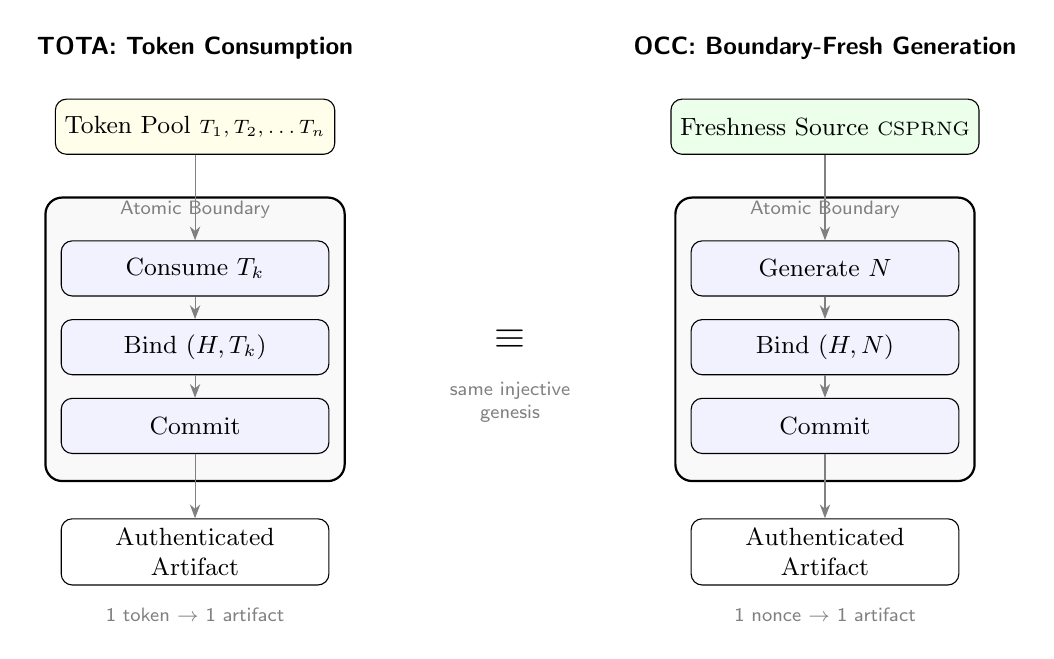
\begin{tikzpicture}[
  box/.style={draw, rounded corners=4pt, minimum width=3.4cm, minimum height=0.7cm,
              align=center, font=\small},
  bndbox/.style={draw, thick, rounded corners=6pt, inner sep=8pt, fill=gray!5},
  arr/.style={-{Stealth[length=5pt]}, gray},
  lbl/.style={font=\scriptsize\sffamily, text=gray},
]
% --- Left column: TOTA ---
\node[font=\small\bfseries\sffamily] (ltitle) at (-4,5.2) {TOTA: Token Consumption};
\node[box, fill=yellow!8] (pool) at (-4,4.2) {Token Pool \scriptsize $T_1, T_2, \ldots T_n$};

\node[bndbox, minimum width=3.8cm, minimum height=3.6cm] (lbnd) at (-4,1.5) {};
\node[lbl] at (-4,3.15) {Atomic Boundary};
\node[box, fill=blue!5] (lcon) at (-4,2.4) {Consume $T_k$};
\node[box, fill=blue!5] (lbind) at (-4,1.4) {Bind $(H, T_k)$};
\node[box, fill=blue!5] (lcommit) at (-4,0.4) {Commit};

\node[box] (lart) at (-4,-1.2) {Authenticated\\Artifact};
\node[lbl] at (-4,-2.0) {1 token $\to$ 1 artifact};

\draw[arr] (pool) -- (lcon);
\draw[arr] (lcon) -- (lbind);
\draw[arr] (lbind) -- (lcommit);
\draw[arr] (lcommit) -- (lart);

% --- Equivalence symbol ---
\node[font=\Large] at (0,1.5) {$\equiv$};
\node[lbl, text width=2cm, align=center] at (0,0.7) {same injective\\genesis};

% --- Right column: OCC ---
\node[font=\small\bfseries\sffamily] (rtitle) at (4,5.2) {OCC: Boundary-Fresh Generation};
\node[box, fill=green!8] (src) at (4,4.2) {Freshness Source \scriptsize CSPRNG};

\node[bndbox, minimum width=3.8cm, minimum height=3.6cm] (rbnd) at (4,1.5) {};
\node[lbl] at (4,3.15) {Atomic Boundary};
\node[box, fill=blue!5] (rgen) at (4,2.4) {Generate $N$};
\node[box, fill=blue!5] (rbind) at (4,1.4) {Bind $(H, N)$};
\node[box, fill=blue!5] (rcommit) at (4,0.4) {Commit};

\node[box] (rart) at (4,-1.2) {Authenticated\\Artifact};
\node[lbl] at (4,-2.0) {1 nonce $\to$ 1 artifact};

\draw[arr] (src) -- (rgen);
\draw[arr] (rgen) -- (rbind);
\draw[arr] (rbind) -- (rcommit);
\draw[arr] (rcommit) -- (rart);
\end{tikzpicture}
\caption{Token--Nonce duality. TOTA (left) consumes a pre-existing token from a finite pool. OCC (right) generates a boundary-fresh value from a cryptographic source. Both enforce the same invariant: each authenticated artifact corresponds to exactly one irreversible authorization event (injective genesis). Collision resistance makes boundary-fresh generation operationally equivalent to token consumption.}
\label{fig:token-nonce}
\end{figure}

The equivalence shown in \cref{fig:token-nonce} is structural, not operational. The reader should resist the interpretation that OCC merely replaces physical tokens with virtual ones. The insight is the reverse: TOTA is a special case of OCC in which the authorization event happens to be reified as a consumable object. OCC reveals that the underlying enforcement primitive is not the token but the structural constraint---that authenticated state is unreachable without an irreversible authorization event at the commit boundary. Tokens enforce this by depletion; boundary-fresh generation enforces it by cryptographic causality. The primitive is the constraint, not the mechanism.

Similarly, the boundary-fresh value $N$ should not be understood as merely a ``nonce for replay protection.'' In conventional protocols, nonces prevent message replay. In OCC, the boundary-fresh value is \emph{the authorization event itself}---its generation inside the boundary constitutes the irreversible act that gates the creation of authenticated state. Producing valid verification material is proof that this act occurred, not merely that a unique value was included.


% --- 6.1 ---
\subsection{Atomic Causality}
\label{sec:atomic-causality}

Under Atomic Causality, three operations are linked into a single indivisible event inside an atomic execution boundary, completed only through a protected commit interface requiring a boundary-held capability:
\begin{enumerate}
  \item \textbf{Authorization}: A boundary-held capability is exercised.
  \item \textbf{Cryptographic binding}: Boundary-fresh output is bound to a content-dependent value.
  \item \textbf{Durable commit}: The authenticated artifact is committed to persistent storage or an output channel.
\end{enumerate}

Authenticated durable state is reachable only if these operations occur together, in order, within the same atomic execution boundary. If any step fails, no authenticated artifact is produced.

% ---------- Figure 2: Atomic Causality ----------
\begin{figure}[htbp]
\centering
\begin{tikzpicture}[
  step/.style={draw, rounded corners=3pt, minimum width=3cm, minimum height=0.65cm,
               align=center, font=\small},
  arr/.style={-{Stealth[length=5pt]}, gray},
  lbl/.style={font=\scriptsize\sffamily, text=gray},
]
% --- Left: OCC Atomic ---
\node[font=\small\bfseries\sffamily] at (-3.8,4) {OCC: Atomic Causality};
\node[draw, thick, rounded corners=6pt, minimum width=3.8cm, minimum height=3.4cm,
      fill=gray!5] (lbox) at (-3.8,1.8) {};
\node[step, fill=green!8] (la) at (-3.8,3.0) {1. Authorize};
\node[step, fill=green!8] (lb) at (-3.8,2.0) {2. Bind};
\node[step, fill=green!8] (lc) at (-3.8,1.0) {3. Commit};
\draw[arr] (la) -- (lb);
\draw[arr] (lb) -- (lc);
\node[lbl] at (-3.8,0.0) {single atomic operation};
\node[font=\large, green!60!black] at (-3.8,-0.5) {\checkmark};

% --- Right: Non-OCC Separated ---
\node[font=\small\bfseries\sffamily] at (3.8,4) {Non-OCC: Separated Steps};
\node[step, fill=red!8] (ra) at (3.8,3.0) {1. Authorize};
\node[step, fill=red!8] (rb) at (3.8,2.0) {2. Bind};
\node[step, fill=red!8] (rc) at (3.8,1.0) {3. Commit};
\draw[arr] (ra) -- (rb);
\draw[arr] (rb) -- (rc);
\node[lbl, text=red!60!black] at (5.8,2.5) {$\leftarrow$ observable gap};
\node[lbl, text=red!60!black] at (5.8,1.5) {$\leftarrow$ observable gap};
\node[font=\large, red!70!black] at (3.8,-0.5) {$\times$};
\end{tikzpicture}
\caption{Atomic Causality versus separated operations. In OCC (left), authorization, binding, and commit occur as a single indivisible event inside the boundary with no externally observable intermediate states. In non-OCC systems (right), these are separate operations with observable gaps exploitable by adversaries.}
\label{fig:atomic-causality}
\end{figure}


% --- 6.2 ---
\subsection{Why This Is Not Attested Execution}
\label{sec:not-attestation}

This enforcement model is not equivalent to conventional attested execution followed by signing. The distinction is precise and consequential.

Attestation-based systems can demonstrate that particular trusted code executed and produced particular signed outputs. This answers the question: \emph{``Was this artifact produced by trusted code?''} But attestation does not answer a different and more fundamental question: \emph{``Could an artifact not produced by trusted code have entered this trust domain through any available commit path?''}

In most attestation-based systems, enforcement is advisory. Trusted processes may produce signed outputs, while untrusted processes may still produce durable state that enters downstream systems through alternative commit paths. The enforcement gap is not in the attested path---it is in the unattested paths that remain open.

Origin Controlled Computing closes this gap. Authenticated durable state is reachable \emph{only} through protected commit paths that enforce atomic binding, authorization, and durable commit at the moment of finalization. Valid verification material implies not merely that trusted code ran, but that \emph{no alternative path to authenticated state exists}. This is a structural property of the commit architecture, not a property of any single attested process.


% --- 6.3 ---
\subsection{Token-Equivalence of Boundary-Fresh Generation}
\label{sec:token-equivalence}

Token-equivalence does not arise from uniqueness alone. It arises from atomic, attested finalization that combines several properties: boundary isolation ensures the fresh output is generated only inside the atomic execution boundary; unpredictability prevents adversaries from predicting or precomputing valid values; binding ties the fresh output to a content-dependent value before commit; a boundary-held authorization capability gates finalization; and attestation or signing produces verification material validatable under accepted trust anchors.

Together, these properties ensure that producing valid verification material implies that a specific authorization event occurred inside the boundary at finalization time. The fresh value $N$ functions as a consumed authorization unit whose existence is cryptographic evidence of an irreversible finalization event---not merely a unique identifier. To be precise: the fresh value alone does not constitute authorization. Authorization arises from the indivisible combination of boundary isolation, capability-gated access, atomic binding, and freshness---no single property is sufficient, and removing any one breaks the enforcement guarantee.

Functionally, the space of possible boundary-fresh outputs acts as an effectively inexhaustible universe of unused authorization units, and generating one during finalization constitutes irreversible consumption. Each accepted artifact necessarily corresponds to exactly one irreducible authorization event, making boundary-fresh outputs operationally equivalent to single-use tokens even without explicit allocation or tracking.


% ============================================================================
% 7. FORMAL MODEL
% ============================================================================
\section{Formal Model}
\label{sec:formal}

We formalize Origin Controlled Computing using a labeled transition system and closure algebra. This formalization captures the essential properties of the architecture and enables precise comparison with existing enforcement models.


% --- 7.1 ---
\subsection{State Space and Transition System}
\label{sec:state-space}

\begin{definition}[OCC System]
\label{def:occ-system}
An OCC system is a labeled transition system $(\Sigma, \rightarrow, E)$ where:
\begin{itemize}
  \item $\Sigma$ is the state space, partitioned into $\Sigauth \cup \Sigunauth$.
  \item ${\rightarrow} \subseteq \Sigma \times E \times \Sigma$ is the transition relation labeled by events $E$.
  \item $\Eauth \subseteq E$ is the set of authorization events.
  \item $\mathcal{C} \subseteq \Sigma \times \Eauth \times \Sigauth$ is the \emph{genesis constructor relation}.
\end{itemize}
\end{definition}

The genesis constructor relation $\mathcal{C}$ captures the protected commit interface: it is the only relation that produces elements of $\Sigauth$. Candidate state in $\Sigunauth$ may be created freely by any process.


% --- 7.2 ---
\subsection{Core Invariants}
\label{sec:core-invariants}

An OCC-compliant system enforces three invariants:

\begin{invariant}[Constructibility --- Closure Property]
\label{inv:constructibility}
\[
  \forall\, s' \in \Sigauth : s' \in \ClC(\Eauth)
\]
where $\ClC(\Eauth) = \{ s' \mid \exists\, s \in \Sigma,\, e \in \Eauth : (s, e, s') \in \mathcal{C} \}$.

Every element of the authenticated state space was produced by a genesis constructor under an authorized event.
\end{invariant}

\begin{invariant}[Constructor Completeness --- Unforgeability]
\label{inv:completeness}
\[
  \forall\, s, s', e :\;
  \bigl(s \xrightarrow{e} s' \;\wedge\; s' \in \Sigauth\bigr)
  \;\Rightarrow\;
  \bigl(e \in \Eauth \;\wedge\; (s, e, s') \in \mathcal{C}\bigr)
\]

All transitions into the authenticated state space are genesis constructors under authorized events. There is no transition into $\Sigauth$ that bypasses $\mathcal{C}$.
\end{invariant}

\begin{invariant}[Atomic Causality --- Indivisibility]
\label{inv:atomic-causality}
\[
  \forall\, (s, e, s') \in \mathcal{C} :\;
  \mathrm{authorize}(e),\; \mathrm{bind}(e),\; \mathrm{commit}(s')
\]
occur in a single atomic transition with no intermediate states observable outside the protected boundary.

Authorization, cryptographic binding, and durable commit are inseparable within the atomic execution boundary.
\end{invariant}


% --- 7.3 ---
\subsection{Authenticated State as Closure Algebra}
\label{sec:closure-algebra}

The authenticated state space $\Sigauth$ forms a \emph{closure space} generated by authorization events through genesis constructors. Formally, define the closure operator:
\[
  \Auth : \mathcal{P}(\Sigma) \rightarrow \mathcal{P}(\Sigma), \quad
  \Auth(S) = \{ s' \mid \exists\, e \in \Eauth,\; s \in S : (s, e, s') \in \mathcal{C} \}
\]

The invariant $\Sigauth = \ClC(\Eauth)$ states that the authenticated state space is exactly the closure under authorized genesis. This makes authentication a \emph{topological property} of the system's state space rather than a local property of individual artifacts.

This formulation connects to existing mathematical structures:
\begin{itemize}
  \item \textbf{Order theory}: $\Sigauth$ forms a Moore family (closed under arbitrary intersections of compliant subsets).
  \item \textbf{Type theory}: Genesis constructors are the sole constructors of an abstract data type; $\Sigauth$ has private constructors.
  \item \textbf{Provenance}: Unlike provenance semirings~\cite{green2007}, which annotate data with origin information, OCC \emph{enforces} that authenticated state can only exist if it has authorized genesis---enforcement, not annotation.
\end{itemize}


% --- 7.4 ---
\subsection{Token--Nonce Duality}
\label{sec:duality}

The Trusted Origin Token Architecture and Origin Controlled Computing enforce the same injective genesis invariant through dual mechanisms:

\begin{definition}[Injective Genesis]
\label{def:injective-genesis}
A system enforces injective genesis if and only if the map $\varphi : \Eauth \rightarrow \Sigauth$ defined by $\varphi(e) = s'$ where $(s, e, s') \in \mathcal{C}$ is an injection. Each authorization event produces at most one authenticated artifact, and each authenticated artifact corresponds to exactly one authorization event.
\end{definition}

\textbf{Token Conservation (TOTA).} Authorization events are reified as consumable tokens. Consumption tracking enforces $|\text{tokens consumed}| = |\Sigauth|$. This is a \emph{depletable resource} model analogous to affine types in linear logic.

\textbf{Boundary-Fresh Uniqueness (OCC).} Authorization events are boundary-generated values whose cryptographic freshness ensures uniqueness. Each value appears in exactly one authenticated artifact. This is a \emph{unique generator} model analogous to existential types with freshness guarantees.

Under perfect cryptography and uncompromised boundary assumptions, these mechanisms are \emph{cryptographic duals}: they enforce the same cardinality constraint $|\Eauth| = |\Sigauth|$ through isomorphic algebraic structures---consumable resources versus generative uniqueness. The token model makes injectivity definitional; the boundary-fresh model makes injectivity derived from collision resistance and freshness guarantees.

\begin{remark}[Structural Non-Reusability]
\label{rem:non-reusability}
Injective genesis ensures that no authorization event can contribute to more than one authenticated artifact, and no authenticated artifact can exist without a unique authorization event. Authorization events are irreversible state transitions---once an event has produced an authenticated artifact, it is permanently consumed by that production and cannot be replayed, redirected, or shared. This is a structural property of the genesis constructor, not a bookkeeping constraint enforced by external tracking.

Readers familiar with distributed ledger systems may recognize an analogy to double-spend prevention. The invariant is similar---$|\Eauth| = |\Sigauth|$ ensures one-to-one correspondence---but the enforcement mechanism is fundamentally different. In ledger systems, double-spend prevention requires global consensus over a shared transaction history. In OCC, non-reusability is enforced locally by the atomic execution boundary: boundary-fresh generation produces a value that is cryptographically bound to exactly one artifact at exactly one finalization event, with no external coordination required.
\end{remark}


% ============================================================================
% 8. SECURITY GAME
% ============================================================================
\section{Adversarial Model and Security Game}
\label{sec:security}

We define a security game that captures the adversarial setting in which Origin Controlled Computing operates.


% --- 8.1 ---
\subsection{Threat Model}
\label{sec:threat-model}

The adversary $\mathcal{A}$ is assumed to possess:
\begin{itemize}
  \item Full control of application code executing outside the atomic execution boundary.
  \item Control of storage systems and network transport.
  \item The ability to replay, substitute, or synthesize candidate data.
  \item Access to all previously produced authenticated artifacts and their verification material.
\end{itemize}

The adversary does \emph{not} possess:
\begin{itemize}
  \item The ability to execute code inside the atomic execution boundary.
  \item Access to boundary-held capabilities (signing keys, capability tokens).
  \item The ability to predict or reproduce boundary-fresh cryptographic output.
\end{itemize}


% --- 8.2 ---
\subsection{Security Game: Origin Forgery}
\label{sec:forgery-game}

\begin{definition}[Origin Forgery Game]
\label{def:forgery-game}
The game $\mathrm{Forge}_{\mathcal{A}}^{\mathrm{OCC}}(\lambda)$ proceeds as follows, where $\lambda$ is the security parameter:
\begin{enumerate}
  \item \textbf{Setup.} The challenger initializes an OCC system with boundary identity $\mathit{id}$, trust anchors $\mathit{TA}$, and security parameter $\lambda$.
  \item \textbf{Query phase.} The adversary $\mathcal{A}$ may submit candidate data to the protected commit interface and observe the resulting authenticated artifacts and verification material. The adversary may make polynomially many such queries.
  \item \textbf{Forgery.} The adversary outputs a candidate artifact $a^*$ and verification material $v^*$.
  \item \textbf{Win condition.} $\mathcal{A}$ wins if:
  \begin{itemize}
    \item $(a^*, v^*)$ verifies under trust anchors $\mathit{TA}$, and
    \item $(a^*, v^*)$ was not produced by any query to the protected commit interface.
  \end{itemize}
\end{enumerate}
\end{definition}

\begin{definition}[OCC Security]
\label{def:occ-security}
An OCC system is \emph{secure} if for all probabilistic polynomial-time adversaries $\mathcal{A}$:
\[
  \Pr[\mathrm{Forge}_{\mathcal{A}}^{\mathrm{OCC}}(\lambda) = 1] \leq \mathrm{negl}(\lambda)
\]
\end{definition}

\begin{proposition}[Security Reduction]
\label{prop:security-reduction}
If the signature scheme is existentially unforgeable under chosen-message attack (EUF-CMA) and the freshness source is collision-resistant, then the OCC system is secure under \cref{def:forgery-game}.
\end{proposition}

\begin{proof}[Proof sketch]
Suppose adversary $\mathcal{A}$ wins the Origin Forgery Game with non-negligible probability. Then $\mathcal{A}$ has produced verification material $(a^*, v^*)$ that validates under trust anchors $\mathit{TA}$ without invoking the protected commit interface. The verification material includes a signature over a binding of boundary-fresh output $N^*$ and a content-dependent value $H^*$. Since $\mathcal{A}$ did not invoke the boundary, either: (a)~$\mathcal{A}$ forged the signature, contradicting EUF-CMA security; or (b)~$\mathcal{A}$ reused a boundary-fresh value $N$ from a previous query with different content, contradicting binding integrity; or (c)~$\mathcal{A}$ replayed an exact $(a, v)$ pair from a previous query, which fails the win condition. Therefore no PPT adversary wins with non-negligible probability.
\end{proof}

This reduction relies on two distinct classes of assumption: cryptographic assumptions (EUF-CMA signature security, collision resistance of the freshness source) and architectural assumptions (boundary isolation, non-extractability of signing keys, atomicity of the commit operation). The cryptographic assumptions are standard and reducible to well-studied hardness problems. The architectural assumptions define the trusted computing base and must be enforced by the boundary implementation; they are not modeled cryptographically but are explicit preconditions of the threat model defined in \cref{sec:security}.


% --- 8.3 ---
\subsection{Falsifiable Distinctions}
\label{sec:falsifiers}

The following tests distinguish OCC-compliant systems from systems that appear similar but fail to enforce origin control.

\paragraph{F1: Post-hoc Annotation.}
If there exists a function $f: \Sigunauth \rightarrow \Sigauth$ that promotes unauthenticated state to authenticated state while preserving content, the system is not OCC-compliant. This test fails for any system where content is created first and authentication is applied afterward---signing, blockchain registration, provenance database entry, or metadata attachment. These are \emph{annotation systems}, not origin enforcement.

\paragraph{F2: Unconfined Constructor.}
If the genesis constructor can be invoked from contexts outside the protected boundary, the system violates constructor completeness. This test fails when signing keys are accessible to application code, when the commit interface is a public API without boundary isolation, or when trusted and untrusted code share execution context.

\paragraph{F3: Authorization Forgery.}
If an adversary without boundary access can produce events $e$ satisfying $\mathrm{authorized}(e) = \mathrm{true}$, the system violates unforgeability. This test fails when signing keys are extractable, when tokens can be synthesized without authority, or when capabilities can be delegated outside the boundary.

\paragraph{F4: Observable Atomicity Break.}
If the genesis transition can be decomposed into externally observable intermediate steps---authorization at time $t_1$, binding at $t_2 > t_1$, commit at $t_3 > t_2$---the system violates Atomic Causality. This test fails for systems where authorization checking, signing, and storage commit are separate API calls, creating time-of-check-to-time-of-use vulnerabilities.

\paragraph{F5: Retroactive Authentication.}
If durable state can be created first and then promoted to authenticated form by any post-hoc operation that preserves content, the system is implementing annotation, not origin control. This is the most direct test: if the content bytes can exist before the authorization event, the system does not enforce OCC.


% ============================================================================
% 9. ARCHITECTURE
% ============================================================================
\section{Architecture}
\label{sec:architecture}


% --- 9.1 ---
\subsection{State Transition Model}
\label{sec:state-transition}

Origin Controlled Computing distinguishes between candidate digital state and authenticated durable state. Candidate state may exist anywhere and may be adversarial. Authenticated durable state consists of externally visible or persistent artifacts whose authenticated form includes verification material produced by enforced finalization.

The transition from candidate to authenticated occurs at \emph{commit paths}: file writes, storage uploads, message publication, model output export, sensor data release, and log entry creation.

This transition is mediated by four architectural components: an atomic execution boundary, boundary-fresh cryptographic computation, a protected commit interface, and a boundary-held capability. Outside the boundary, systems may generate arbitrary data. The authenticated durable form is unreachable without successful finalization.

% ---------- Figure 3: State Transition Model ----------
\begin{figure}[htbp]
\centering
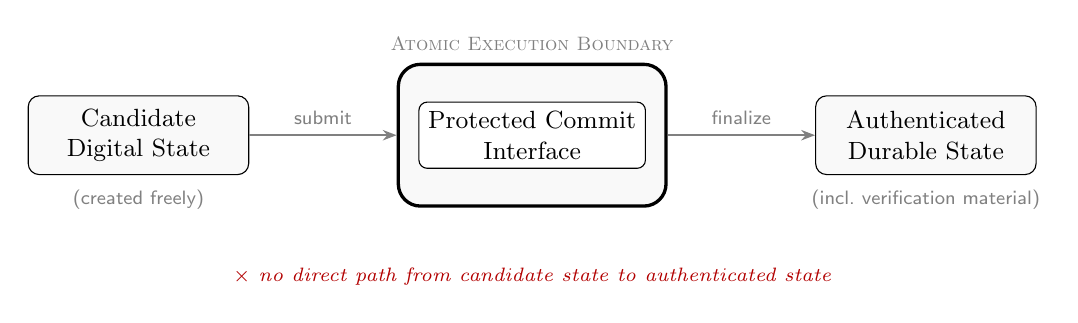
\begin{tikzpicture}[
  box/.style={draw, rounded corners=4pt, minimum width=2.8cm, minimum height=1cm,
              align=center, font=\small, fill=gray!5},
  bnd/.style={draw, very thick, rounded corners=8pt, minimum width=3.4cm,
              minimum height=1.8cm, fill=gray!5, align=center},
  arr/.style={-{Stealth[length=5pt]}, gray, thick},
  lbl/.style={font=\scriptsize\sffamily, text=gray},
]
\node[box] (cand) at (0,0) {Candidate\\Digital State};
\node[lbl, below=2pt of cand] {(created freely)};
\node[bnd] (bnd) at (5,0) {};
\node[lbl, above=1pt] at (bnd.north) {\textsc{Atomic Execution Boundary}};
\node[draw, rounded corners=3pt, fill=white, minimum width=2.4cm, font=\small,
      align=center] (pci) at (5,0) {Protected Commit\\Interface};
\node[box] (auth) at (10,0) {Authenticated\\Durable State};
\node[lbl, below=2pt of auth] {(incl.\ verification material)};

\draw[arr] (cand) -- node[above, lbl] {submit} (bnd);
\draw[arr] (bnd) -- node[above, lbl] {finalize} (auth);

\node[font=\scriptsize\itshape, red!70!black] at (5,-1.8)
  {$\times$ no direct path from candidate state to authenticated state};
\end{tikzpicture}
\caption{State transition model. Authenticated durable state is reachable only through the protected commit interface inside the atomic execution boundary. No direct path from candidate state to authenticated state exists.}
\label{fig:state-transition}
\end{figure}


% --- 9.2 ---
\subsection{Atomic Finalization Protocol}
\label{sec:finalization-protocol}

Atomic finalization proceeds as a single ordered operation:
\begin{enumerate}
  \item Candidate state is prepared outside the boundary.
  \item The request enters the protected commit interface and crosses into the atomic execution boundary.
  \item Boundary-fresh cryptographic output $N$ is generated.
  \item A content-dependent value $H$ is computed (e.g., a cryptographic hash of the artifact).
  \item Binding material is produced over $(H, N)$.
  \item Authorization is performed using a boundary-held capability.
  \item Authenticated durable state and verification material are committed.
\end{enumerate}

If any step fails, no authenticated durable state is produced. The system is \emph{fail-closed}: failures prevent authenticated creation rather than producing ambiguous or partially authenticated outputs.


% --- 9.3 ---
\subsection{Verification Model}
\label{sec:verification-model}

Verification relies on cryptographic attestation produced by the atomic execution boundary over the binding between content and boundary-fresh output. Concretely, the boundary produces verification material covering: the content-dependent value $H$, the boundary-fresh output $N$, and optional policy or context metadata. This material is signed or attested using boundary-held cryptographic keys.

Verifiers accept artifacts only if the verification material validates under approved trust anchors, which may include pinned boundary public keys, manufacturer or platform roots certifying boundary identities, or signed domain policy manifests specifying acceptable boundary identities, epochs, and validity windows.

No registry of artifacts is required. Verifiers need not identify the producing application---only that the artifact could not have been finalized outside an approved boundary under accepted policy.


% --- 9.4 ---
\subsection{Enforcement and Verification Are Separate Architectural Layers}
\label{sec:enforcement-verification}

A distinction fundamental to OCC must be stated explicitly. Enforcement determines whether authenticated durable state \emph{exists}. Verification determines whether a third party can \emph{demonstrate} that authenticated durable state exists. These are different properties operating at different architectural layers.

Enforcement is irrevocable. Once candidate state has been finalized through the protected commit interface---once authorization, binding, and durable commit have occurred as a single atomic event inside the boundary---the resulting artifact is authenticated. This is a historical fact about the artifact's genesis, not a claim that depends on the continued availability of any proof material.

Verification is operationally contingent. A verifier can confirm an artifact's authenticated status only if verification material is accessible---either co-traveling with the artifact or retrievable from a reference point. If all copies of verification material are lost, the artifact becomes \emph{unverifiable} but does not become \emph{unauthenticated}. The genesis event still occurred. The enforcement invariants still held at the moment of creation. The artifact's authenticated status is a property of its creation path, not a property of currently available evidence.

This separation is what distinguishes OCC from verification systems, provenance frameworks, and attestation protocols. Those systems define authenticity in terms of what can currently be checked. OCC defines authenticity in terms of what was structurally enforced at creation. Verification is one mechanism for observing the consequences of enforcement, but it is not the enforcement itself.


% --- 9.5 ---
\subsection{Verification Independence from Proof Transport}
\label{sec:verification-independence}

A critical architectural property of OCC is that the enforcement invariants described in \cref{sec:invariants} hold at genesis and are not contingent on any subsequent verification event, proof transport mechanism, or reference infrastructure availability. Verification is a mechanism for demonstrating that enforcement occurred. It is not a component of enforcement.

The verification model is therefore independent of how verification material reaches the verifier. OCC supports multiple verification models, and the choice among them is a deployment decision, not an architectural constraint. No verification model choice affects whether the enforcement invariants hold.

\paragraph{Portable proof.}
Verification material travels with the artifact---embedded in file metadata, carried in a sidecar file, or included in a manifest bundle. This is compatible with existing provenance formats such as C2PA and enables self-contained verification without external dependencies.

\paragraph{Reference-based verification.}
Verification material is held at one or more canonical reference points operated by the producing boundary, a trusted third party, or a federated network. When a verifier encounters an artifact without co-traveling proof, the verifier computes the artifact's content hash and queries the reference point to obtain the verification material produced at genesis. The artifact carries nothing. Its content hash is its lookup key.

\paragraph{Hybrid verification.}
Artifacts carry verification material when the distribution channel preserves it. Reference points serve as authoritative fallback for stripped, reformatted, or re-distributed artifacts. Both modes validate against the same trust anchors and enforce the same invariants.

% ---------- Figure 4: Verification Independence ----------
\begin{figure}[htbp]
\centering
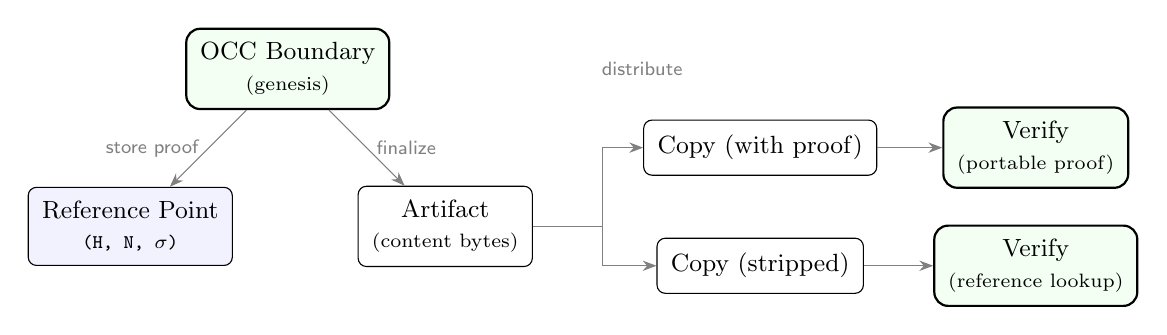
\begin{tikzpicture}[
  box/.style={draw, rounded corners=3pt, minimum height=0.7cm, align=center,
              font=\small, inner sep=5pt},
  bndbox/.style={draw, thick, rounded corners=5pt, fill=green!5, minimum height=0.7cm,
                 align=center, font=\small, inner sep=5pt},
  refbox/.style={draw, rounded corners=3pt, fill=blue!5, minimum height=0.7cm,
                 align=center, font=\small, inner sep=5pt},
  arr/.style={-{Stealth[length=5pt]}, gray},
  lbl/.style={font=\scriptsize\sffamily, text=gray},
]
% Origin boundary
\node[bndbox] (origin) at (0,2) {OCC Boundary\\{\scriptsize (genesis)}};

% Two outputs
\node[refbox] (ref) at (-2,0) {Reference Point\\{\scriptsize\texttt{(H, N, $\sigma$)}}};
\node[box] (art) at (2,0) {Artifact\\{\scriptsize (content bytes)}};

\draw[arr] (origin) -- node[left, lbl] {store proof} (ref);
\draw[arr] (origin) -- node[right, lbl] {finalize} (art);

% Distribution
\node[box] (copy1) at (6,1) {Copy (with proof)};
\node[box] (copy2) at (6,-0.5) {Copy (stripped)};
\node[bndbox] (v1) at (9.5,1) {Verify\\{\scriptsize (portable proof)}};
\node[bndbox] (v2) at (9.5,-0.5) {Verify\\{\scriptsize (reference lookup)}};

\draw[arr] (art) -- ++(2,0) |- (copy1);
\draw[arr] (art) -- ++(2,0) |- (copy2);
\draw[arr] (copy1) -- (v1);
\draw[arr] (copy2) -- (v2);

\node[lbl] at (4.5,2) {distribute};
\end{tikzpicture}
\caption{Verification independence from proof transport. Artifacts may carry verification material (top path) or be verified by reference lookup using the content hash (bottom path). Both paths validate against the same trust anchors. Authentication survives metadata stripping, format conversion, and redistribution.}
\label{fig:verification-independence}
\end{figure}

This property has significant practical consequences. OCC-authenticated artifacts can be freely copied, reformatted, compressed, transcoded, or distributed through channels that strip metadata---and their authenticated status is permanent regardless of what happens to metadata during distribution. \emph{Verifiability}---the ability for a third party to confirm authenticated status---requires that either co-traveling proof or a reference point is available and that the content-preserving hash can be recomputed. But the artifact's authenticated status, as defined by the enforcement invariants, is an irrevocable consequence of its genesis and does not depend on proof availability. This is a structural advantage over systems that embed provenance in format-specific metadata, which is routinely stripped by social media platforms, content delivery networks, messaging applications, and file conversion tools.

This property is particularly consequential in delay-tolerant and interplanetary networks, where verification material must travel with the data and no return channel to the origin may exist at verification time.

A clarification regarding content transforms is warranted. Verification depends on recomputing a content-dependent hash that matches the hash bound at genesis. Lossless operations that preserve byte-identical content---copying, re-hosting, metadata stripping, container rewrapping---leave this hash intact and verification proceeds directly. Lossy transforms---recompression, transcoding, cropping, resolution scaling---alter the content bytes and therefore invalidate the original binding. Under OCC, a lossy transform produces new candidate state. If the transformed output must itself be authenticated, it requires a new finalization event at a protected transform boundary, producing fresh verification material for the new content. This is not a limitation but a correct application of the enforcement model: the transformed artifact is a different artifact with a different origin. Systems requiring verification across lossy transforms may define robust or perceptual digest schemes as the content-dependent value $H$, but such schemes introduce their own security trade-offs and are a deployment choice, not an architectural requirement. The enforcement invariant is the same regardless of digest construction.

A reference point is not an artifact registry. A registry implies centralized control over all authenticated artifacts and creates a single point of failure for the entire system. A reference point is a service that holds verification material produced by a specific boundary and can be replicated, federated, or operated by the producing boundary itself. Multiple reference points can hold verification material for the same artifact. The trust model does not change: verifiers validate against trust anchors, not against the reference point's authority. Reference points play no role in the enforcement layer. They do not participate in genesis, do not confer authenticated status, and their unavailability does not retroactively affect the authenticated status of any artifact. They are verification infrastructure, not enforcement infrastructure.

% ---------- Figure 5: Verification Structure ----------
\begin{figure}[htbp]
\centering
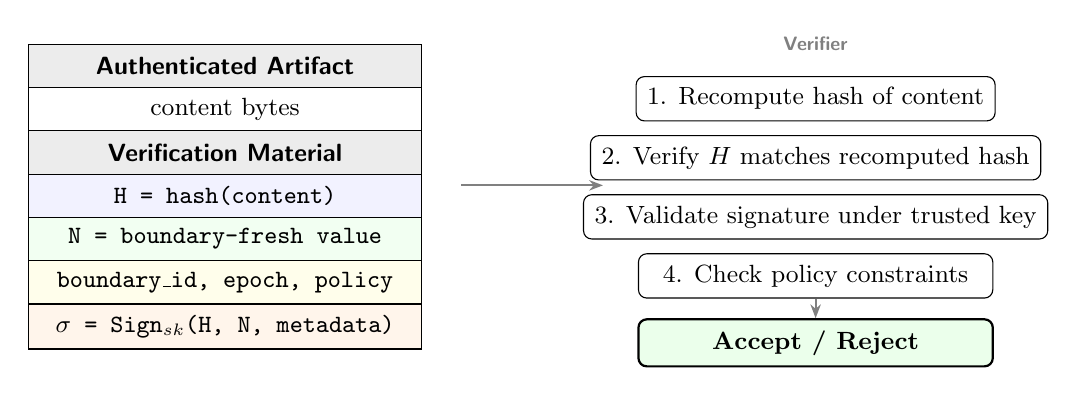
\begin{tikzpicture}[
  cell/.style={draw, minimum width=5cm, minimum height=0.55cm, font=\small,
               anchor=north, align=center, inner sep=4pt},
  hdr/.style={cell, fill=gray!15, font=\small\bfseries\sffamily},
  vstep/.style={draw, rounded corners=3pt, minimum width=4.5cm, minimum height=0.55cm,
                font=\small, align=center, inner sep=4pt},
  arr/.style={-{Stealth[length=5pt]}, gray, thick},
  lbl/.style={font=\scriptsize\sffamily, text=gray},
]
% --- Artifact structure ---
\node[hdr] (ah) at (0,0) {\textsc{Authenticated Artifact}};
\node[cell] (c1) at (0,-0.55) {content bytes};
\node[hdr] (vh) at (0,-1.1) {\textsc{Verification Material}};
\node[cell, fill=blue!5] (v1) at (0,-1.65) {\texttt{H = hash(content)}};
\node[cell, fill=green!5] (v2) at (0,-2.2) {\texttt{N = boundary-fresh value}};
\node[cell, fill=yellow!8] (v3) at (0,-2.75) {\texttt{boundary\_id, epoch, policy}};
\node[cell, fill=orange!8] (v4) at (0,-3.3) {\texttt{$\sigma$ = Sign$_{sk}$(H, N, metadata)}};

% --- Verifier steps ---
\node[lbl] at (7.5,0) {\textbf{Verifier}};
\node[vstep] (s1) at (7.5,-0.7) {1. Recompute hash of content};
\node[vstep] (s2) at (7.5,-1.45) {2. Verify $H$ matches recomputed hash};
\node[vstep] (s3) at (7.5,-2.2) {3. Validate signature under trusted key};
\node[vstep] (s4) at (7.5,-2.95) {4. Check policy constraints};
\node[vstep, fill=green!8, thick] (acc) at (7.5,-3.8) {\textbf{Accept / Reject}};

\draw[arr] (3,-1.8) -- (4.8,-1.8);
\draw[arr] (s4) -- (acc);
\end{tikzpicture}
\caption{Verification structure (portable proof model). An authenticated artifact carries its verification material. In the reference-based model (\cref{fig:verification-independence}), verification material is held separately and retrieved by content hash. The verification checks are identical in both cases.}
\label{fig:verification-structure}
\end{figure}


% --- 9.6 ---
\subsection{Boundary Compromise and Recovery}
\label{sec:boundary-compromise}

If the atomic execution boundary or its signing keys are compromised, the system cannot distinguish forged authenticated artifacts from legitimate ones under that boundary identity. Trust collapses to the compromised boundary, not to the entire system. Recovery is handled operationally by revoking or rotating trust anchors, introducing new boundary identities, and enforcing epoch or policy constraints on acceptable verification material. No artifact registry or retroactive correction mechanism is required.

The critical architectural property is that \emph{enforcement strength scales with key isolation strength}. Software boundaries provide enforcement convenience and deployment accessibility but are inherently weaker against key extraction. Hardware-backed boundaries---secure enclaves, HSMs, trusted execution environments---provide structural guarantees by enforcing both key non-extractability and constrained usage semantics.


% --- 9.7 ---
\subsection{Security Properties}
\label{sec:security-properties}

\begin{property}[Non-Retroactivity]
\label{prop:non-retroactivity-arch}
Authenticated durable state cannot be produced after the fact for pre-existing data.
\end{property}

\begin{property}[Creation-Path Exclusivity]
\label{prop:creation-path}
Authenticated durable state is structurally reachable only through the protected commit interface and cannot be produced by any alternative code path or post-hoc process.
\end{property}

\begin{property}[Content Integrity]
\label{prop:content-integrity}
Verification material binds authenticated state to specific content bytes.
\end{property}

\begin{property}[Replay Resistance]
\label{prop:replay-resistance}
Boundary-fresh cryptographic output prevents reuse of prior authorization events.
\end{property}


% ============================================================================
% 10. RELATED WORK
% ============================================================================
\section{Related Work}
\label{sec:related}

Origin Controlled Computing intersects with several established areas of security and systems research. This section distinguishes OCC from the most closely related approaches and identifies the specific enforcement gap each leaves open.


% --- 10.1 ---
\subsection{Attested Execution and Trusted Execution Environments}
\label{sec:tees}

Trusted Execution Environments (TEEs) such as Intel SGX, Intel TDX, and ARM Confidential Compute Architecture (CCA) provide hardware-isolated execution with remote attestation. The DICE (Device Identifier Composition Engine) architecture establishes device identity through layered measurements. The IETF RATS (Remote ATtestation procedureS) framework standardizes attestation evidence formats and verification workflows.

These systems answer the question: \emph{``Did specific trusted code execute?''} OCC asks a different question: \emph{``Is authenticated durable state reachable only through enforced commit paths?''} Attestation authenticates a pipeline. OCC constrains the commit architecture so that alternative pipelines cannot produce authenticated state. TEEs are one possible implementation substrate for OCC boundaries, but attestation alone does not close unprotected commit paths that exist alongside the attested process.


% --- 10.2 ---
\subsection{Content Provenance and Credential Systems}
\label{sec:provenance-systems}

The Coalition for Content Provenance and Authenticity (C2PA) and related provenance standards define how to represent claims about an artifact's origin, edits, and attribution, and how to transport that information across tools and platforms. When a signed artifact is present, these standards make integrity and lineage verifiable and interoperable.

OCC targets a different architectural layer. Provenance standards are a \emph{packaging and disclosure layer}: they define what claims look like and how to verify them. OCC is an \emph{enforcement layer}: it determines whether authenticated durable state can be finalized at all unless creation-time conditions were met. The distinction matters because provenance ecosystems are voluntary at the edges. A signed artifact can be verified, but an unsigned artifact can still be created, circulated, and injected into downstream systems that do not strictly require provenance at every boundary. Provenance improves traceability without guaranteeing exclusion.

OCC and provenance are complementary. OCC strengthens provenance by making provenance verifiability a prerequisite for admission into protected domains. Provenance remains the interoperability layer that carries claims across ecosystems; OCC supplies the mechanism by which systems enforce that only authenticated artifacts become trusted durable state. Under OCC with reference-based verification, provenance survives even when manifests are stripped during distribution (see the provenance example in \cref{sec:provenance-example} and the verification model in \cref{sec:verification-independence}).


% --- 10.3 ---
\subsection{Reference Monitors and Access Control}
\label{sec:reference-monitors}

The classical reference monitor concept (Anderson, 1972) mediates all operations on existing objects: every access is checked against a policy before it is permitted. Origin Controlled Computing is strictly stronger in one dimension: it controls not merely which \emph{operations} on objects are permitted, but which \emph{objects are permitted to exist} in authenticated form. Classical access control assumes object creation is uncontrolled and focuses on subsequent access. OCC constrains creation itself.

Formally, a reference monitor enforces:
\[
  \forall\, \mathit{op} \in \mathit{Operations},\;
  \forall\, \mathit{obj} \in \mathit{Objects} :
  \mathit{execute}(\mathit{op}, \mathit{obj})
  \Rightarrow
  \mathit{authorized}(\mathit{subject}, \mathit{op}, \mathit{obj})
\]
A genesis monitor (OCC) enforces:
\[
  \forall\, \mathit{obj} \in \Sigauth :
  \mathit{obj} \in \Sigma
  \Rightarrow
  \exists\, e \in \Eauth :
  \mathit{genesis}(\mathit{obj}) = \mathcal{C}(e, \mathit{data})
\]
The key difference: a reference monitor assumes objects exist and mediates access. A genesis monitor constrains which authenticated objects can exist at all. This is \emph{mandatory constructor security}, analogous to mandatory access control but applied to object generation rather than object access.


% --- 10.4 ---
\subsection{Capability-Based Security}
\label{sec:capability}

Object-capability models (Dennis \& Van Horn, 1966; Miller, 2006) enforce that access to objects requires possession of an unforgeable capability. Membrane patterns in capability systems create revocable boundaries around object graphs.

OCC shares the emphasis on structural enforcement through unforgeable references but applies it at a different layer. Capabilities control \emph{reachability of existing objects}. OCC controls \emph{constructibility of new authenticated state}. The boundary-held capability in OCC is a capability-security mechanism, but the enforcement target---preventing existence rather than preventing access---distinguishes OCC from classical capability models.


% --- 10.5 ---
\subsection{Information Flow Control}
\label{sec:ifc}

Mandatory information flow control (Goguen \& Meseguer, 1982; Myers \& Liskov, 1997) constrains how information propagates through a system. OCC enforces a related but distinct property: it constrains how authenticated state is \emph{generated}, not how information flows between existing states. In information flow terms, OCC enforces a mandatory creation policy: authenticated state can only be generated through specific channels (the protected commit interface), analogous to noninterference applied to creation rather than observation.


% --- 10.6 ---
\subsection{Blockchain and Distributed Consensus}
\label{sec:blockchain}

Blockchain systems enforce that state changes require consensus among distributed participants. The architectural parallel to OCC is real: both create structural bottlenecks through which state transitions must pass. However, blockchain achieves consensus through economic coordination among mutually distrustful parties, while OCC achieves origin enforcement through boundary isolation and cryptographic causality at a single enforcement point. OCC generalizes the structural bottleneck principle to arbitrary protected boundaries without requiring distributed consensus, economic incentives, or global coordination.


% --- 10.7 ---
\subsection{Delay-Tolerant Networking and Interplanetary Protocols}
\label{sec:dtn}

The Bundle Protocol (RFC~9171) and DTN architecture provide store-and-forward transport for environments with extreme latency and intermittent connectivity. Bundle security (BPSec, RFC~9172) provides integrity and confidentiality at the bundle layer but does not constrain how authenticated payloads are created---it secures transport, not genesis. OCC complements DTN by enforcing that bundle payloads finalized through a protected commit interface carry portable verification material validatable offline against pre-distributed trust anchors, with no return path to the origin required. OCC proofs map onto BP extension blocks, enabling authenticated bundles to traverse existing DTN infrastructure without routing modifications.


% --- 10.8 ---
\subsection{Summary of Structural Distinctions}
\label{sec:structural-distinctions}

\Cref{tab:comparison} summarizes the structural properties that distinguish OCC from related approaches. Each property is defined by the system invariants and falsifiability tests in \cref{sec:invariants,sec:falsifiers}. Entries reflect architectural constraints, not implementation quality.

\begin{table}[htbp]
\centering
\caption{Structural property comparison across enforcement paradigms.}
\label{tab:comparison}
\small
\begin{tabular}{@{}lccccc@{}}
\toprule
\textbf{Property} &
\textbf{Digital} &
\textbf{TEE /} &
\textbf{Provenance} &
\textbf{Blockchain /} &
\textbf{OCC} \\
& \textbf{Signing} & \textbf{Attested Exec.} & \textbf{(C2PA)} & \textbf{Ledger} & \\
\midrule
Enforces creation-path exclusivity
  & No & No\textsuperscript{a} & No & No & \textbf{Yes} \\
Prevents post-hoc auth.\ wrapping
  & No & No & No & No & \textbf{Yes} \\
Binds authorization to commit atomically
  & No & Partial\textsuperscript{b} & No & Partial\textsuperscript{c} & \textbf{Yes} \\
Proof survives metadata stripping
  & No & No & No & Yes\textsuperscript{d} & \textbf{Yes}\textsuperscript{e} \\
Requires registry or ledger infrastructure
  & No & No & No & Yes & \textbf{No} \\
Enforces admission control (not traceability)
  & No & No & No & No & \textbf{Yes} \\
\bottomrule
\end{tabular}

\medskip
{\scriptsize
\textsuperscript{a}\,TEEs attest that trusted code executed but do not close alternative commit paths to durable state (\cref{sec:concrete-example}).\\
\textsuperscript{b}\,Authorization and execution are attested, but binding and durable commit are typically separate operations.\\
\textsuperscript{c}\,Consensus binds state transitions but does not constrain artifact genesis prior to ledger submission.\\
\textsuperscript{d}\,Ledger entries persist independently, but the artifact-to-ledger binding is established post-creation.\\
\textsuperscript{e}\,Under reference-based verification (\cref{sec:verification-independence}).
}
\end{table}


% ============================================================================
% 11. WORKED EXAMPLES
% ============================================================================
\section{Worked Examples}
\label{sec:examples}

We present two worked examples demonstrating Origin Controlled Computing in distinct domains. In each case, the same architectural pattern applies: candidate data is prepared freely; authenticated durable state is produced only through the protected commit interface; and any artifact not finalized through the boundary is rejected as unauthenticated.


% --- 11.1 ---
\subsection{Secure Media Capture}
\label{sec:media-capture}

Consider a device capturing photos or video for evidentiary or provenance-sensitive use.

Candidate image or video data is produced by the camera sensor and image processing pipeline. This data may exist in memory or temporary buffers. It is not authenticated.

When a capture is to be finalized, the device invokes the protected commit interface for media output. Inside the atomic execution boundary:
\begin{enumerate}
  \item A boundary-fresh value $N$ is generated.
  \item A hash $H$ of the media content is computed.
  \item Verification material is produced by signing over $(H, N)$ together with device identity and capture metadata.
  \item Authorization is performed using a boundary-held capability.
  \item The media file and verification material are committed to durable storage.
\end{enumerate}

Downstream verifiers validate the content hash against the received media, check verification material under approved device or platform trust anchors, and enforce any applicable policy constraints on capture devices or environments.

Any media not finalized through this boundary cannot produce valid verification material and is rejected as unauthenticated---even if it is visually or byte-identical to an authenticated capture. Critically, the system architecture ensures that no other code path---including the application layer, the operating system, or the storage subsystem---can produce artifacts that satisfy verification. The boundary is not merely the preferred creation path; it is the only creation path for authenticated media.


% --- 11.2 ---
\subsection{AI Output Export Pipeline}
\label{sec:ai-pipeline}

Consider an AI inference service exporting model outputs to downstream consumers.

Candidate outputs are produced by model execution and may exist in memory or temporary buffers. They are not authenticated.

When an output is to be released, the system invokes the protected commit interface for output export. Inside the atomic execution boundary:
\begin{enumerate}
  \item A boundary-fresh value $N$ is generated.
  \item A hash $H$ of the output is computed.
  \item Verification material is produced by signing over $(H, N)$ together with model identity and policy metadata.
  \item Authorization is performed using a boundary-held capability.
  \item The output and verification material are committed.
\end{enumerate}

Downstream verifiers validate the content hash, check verification material under approved trust anchors, and enforce policy constraints on acceptable model identities and metadata.

Any AI output not finalized through this boundary cannot produce valid verification material and is rejected as unauthenticated---even if it is byte-identical to an authenticated output. The system architecture ensures that no alternative export path---including direct database writes, API bypasses, or file system access---can produce outputs that satisfy verification. This is particularly relevant for regulatory compliance frameworks such as the EU AI Act, which require AI-generated content to be identifiable. OCC provides an enforcement mechanism rather than a voluntary labeling scheme.


% ============================================================================
% 12. INSTANTIATIONS
% ============================================================================
\section{Instantiations of the Atomic Boundary}
\label{sec:instantiations}

The atomic execution boundary is an architectural abstraction. Concrete implementations vary by platform, deployment environment, and assurance requirements. Possible instantiations include:
\begin{itemize}
  \item \textbf{Device-level TEEs or secure enclaves} gating camera output, sensor release, or local file creation.
  \item \textbf{Kernel-mediated commit paths} controlling writes to protected namespaces.
  \item \textbf{HSM-backed services} finalizing logs, media, or datasets in backend systems.
  \item \textbf{Operating system services} that mediate all protected commit paths, centralizing admission policy and proof generation.
  \item \textbf{Gateway or pipeline enforcement} at ingestion points where data enters trusted domains.
  \item \textbf{Secure pipeline stages} in CI/CD or regulated data ingestion workflows.
\end{itemize}

These mechanisms differ in construction, but the enforcement invariant is the same: authenticated durable state can be finalized only through a protected commit interface that performs boundary-fresh cryptographic binding and authorization inside an atomic execution boundary.

What is required is not a particular trust anchor or hardware feature, but structural enforcement of finalization ordering and exclusivity. The architecture does not prescribe implementations---it defines the invariant that implementations must satisfy.

In practical terms, the protected commit interface presents a narrow surface: the caller submits candidate content and policy metadata; the boundary performs hashing, binding, authorization, and signing internally; and the caller receives the authenticated artifact and its verification material (or a confirmation that verification material has been stored at a reference point keyed by content hash). The caller never handles signing keys, never observes intermediate cryptographic state, and cannot influence the boundary-fresh value. Whether this interface is realized as a system call, a hardware enclave entry point, an HSM API, or a cloud service endpoint, the enforcement properties are identical.

OCC does not prevent the construction of unauthorized boundaries. Any party can build a boundary and produce verification material. However, artifacts produced by unauthorized boundaries fail verification under accepted trust anchors, because those boundaries' identities are not in the approved set. Trust is mediated by trust anchor policy, not by preventing the existence of alternative boundaries.

In practice, layered deployment is common. A device may generate creation-time verification material, while a gateway enforces admission policy and rejects unauthenticated artifacts. Both layers implement the same enforcement principle at different points in the system.


% --- 12.1 ---
\subsection{Enforcement Tier Semantics}
\label{sec:enforcement-tiers}

Concrete instantiations of the atomic execution boundary differ in the strength of the enforcement guarantee they provide. Not all boundaries are equivalent: a software boundary running in process memory and a hardware enclave with remote attestation both produce cryptographically valid verification material, but they provide fundamentally different assurance that the enforcement invariants actually held. This distinction must be made explicit in the proof structure itself.

OCC proofs carry two orthogonal attestations. The first is a \emph{cryptographic attestation}: the signature and public key establish who signed and that the signed content was unaltered. This is machine-checkable by any party with the public key and is unconditionally verifiable offline. The second is an \emph{enforcement attestation}: the boundary's identity measurement and optional platform attestation report establish \emph{under what conditions} signing was permitted---whether the commit gate, key management, nonce generation, and signing occurred inside a verified hardware boundary or merely inside a software process. Atomic causality lives in the second attestation, not the first. A signature proves who signed; the enforcement context proves whether the creation-time constraints of OCC actually held.

Three enforcement tiers capture the practically relevant points in this assurance space:

\begin{definition}[Enforcement Tiers]
\label{def:enforcement-tiers}
Let $B$ be a boundary implementation. The \emph{enforcement tier} of $B$ is a declaration of the structural properties of its atomic execution boundary:
\begin{itemize}
  \item \textbf{Software-only} ($\tau_{\mathrm{sw}}$). The commit gate, signing key, nonce source, and counter are all held in ordinary process memory. No hardware isolation separates them from application code. The signing key may be extractable by any code with sufficient privilege. Verification material is cryptographically valid but provides no hardware boundary guarantee. Suitable for development and integration testing; does not satisfy the Boundary Isolation invariant (\cref{def:aeb}) against a privileged-process adversary.

  \item \textbf{Hardware-bound key} ($\tau_{\mathrm{hw}}$). The signing key is held in a hardware security boundary (Secure Enclave, TPM, HSM) and is non-exportable. However, the commit gate---the logic that decides which candidate data is eligible for signing---runs outside the measured boundary. The host process feeds content digests to the hardware for signing; the hardware signs whatever it is asked. This provides hardware-bound identity: the signing key cannot be extracted, so signatures are unforgeable. But it does not provide causal enforcement: a compromised host can submit arbitrary digests and receive valid signatures without passing through the protected commit interface. The enforcement invariant holds for key security but not for commit-path exclusivity.

  \item \textbf{Measured TEE} ($\tau_{\mathrm{tee}}$). The commit gate, key management, nonce generation, monotonic counter, and signing all execute inside the attested enclave boundary. The host is treated as untrusted and cannot influence the commit decision or observe intermediate cryptographic state. The enclave's identity is a hardware-measured value---a cryptographic hash of the enclave binary computed by the hardware boot chain---that cannot be forged by user-space code or produced by a different binary. A verifier who pins acceptable measurements to a known-good enclave image and validates the attestation report is guaranteed, under the hardware trust model, that the enforcement invariants held at genesis.
\end{itemize}
\end{definition}

A critical subtlety distinguishes tamper-evidence from self-authentication. The enforcement tier is included in the signed body of every OCC proof, making it tamper-evident in transit: an adversary who intercepts a proof and attempts to substitute a higher-assurance tier will break the signature. However, the tier field is \emph{self-reported} by the boundary adapter. A malicious or misconfigured adapter can declare any tier. The signed field prevents downgrade attacks during transmission; it does not prevent a lying producer.

Actual trust in a declared tier therefore requires independent corroboration. For $\tau_{\mathrm{tee}}$, this means: (1)~pinning acceptable measurements to a known-good enclave image hash published by the boundary operator or auditor, and (2)~validating a hardware attestation report---a vendor-signed document generated by the hardware itself, bound to the specific commit, that certifies the enclave measurement matches a known image. Signature verification establishes cryptographic integrity. Measurement pinning establishes identity. Attestation report validation establishes that the identity was produced by real hardware under the declared conditions. All three are necessary; any two leave a gap. A verifier who checks the signature and trusts the self-reported tier without verifying measurement and attestation has verified fact~(A)---who signed---but not fact~(B)---whether the OCC invariants actually held.

\begin{remark}[Hardware-Bound Key is Not Causal Enforcement]
\label{rem:hw-not-causal}
The $\tau_{\mathrm{hw}}$ tier corresponds to devices such as mobile Secure Enclaves, TPMs, or HSMs where the signing key is hardware-protected but the commit gate runs in application code. Such systems provide meaningful security against key extraction---an adversary cannot steal the private key---but do not satisfy commit-path exclusivity. Application code feeding arbitrary digests to the hardware signer can produce valid signatures for any content without traversal of the protected commit interface. This is useful as an identity anchor and may be sufficient for some deployment contexts, but it is architecturally distinct from $\tau_{\mathrm{tee}}$ and does not satisfy OCC's Atomic Causality invariant (\cref{sec:atomic-causality}) against a compromised-host adversary.
\end{remark}

This taxonomy is not a quality ranking among implementations---a $\tau_{\mathrm{sw}}$ boundary is fully correct for development environments where the adversary model does not include privileged process access. It is a structural classification that makes the adversary model explicit in the proof itself. Verifiers select the tier they require based on their own threat model. A local development tool may accept $\tau_{\mathrm{sw}}$. A regulated ingestion gateway may require $\tau_{\mathrm{tee}}$ with measurement pinning and attestation validation. The same proof format and verification protocol supports all three, with enforcement strength determined by verifier policy rather than proof format version.


% ============================================================================
% 13. ADMISSION
% ============================================================================
\section{Admission of Pre-Existing Data}
\label{sec:admission}

Origin Controlled Computing defines authenticity in terms of enforced finalization events, not in terms of historical existence of content bytes.

Candidate data may exist prior to authenticated finalization and may be externally sourced, duplicated, replayed, or synthesized. Such prior existence is outside the trust model and carries no authenticity semantics.

Authenticated durable state is created only when candidate data is finalized through the protected commit interface and bound to boundary-fresh cryptographic output produced inside the atomic execution boundary. Without this enforced finalization event, no artifact can enter authenticated state, regardless of its prior history or method of creation.

The same content may be finalized multiple times in separate authorization events, each producing distinct verification material. Each such event constitutes an independent origin---a distinct enforced admission into authenticated durable state.

Authenticity therefore reflects structural reachability through enforced commit paths, not claims about when or how content bytes first came into existence.


% --- 13.1 ---
\subsection{Enforced Provenance Chains}
\label{sec:provenance-chains}

When content traverses multiple OCC-enforced boundaries, each boundary produces independent verification material for the same content. The result is a structurally enforced provenance chain: an ordered sequence of admission events, each cryptographically bound to the content at its respective boundary. Unlike voluntary provenance annotations, each link in this chain is the product of an enforced finalization event and could not have been produced without traversing the corresponding boundary.

% ---------- Figure 6: Enforced Provenance Chains ----------
\begin{figure}[htbp]
\centering
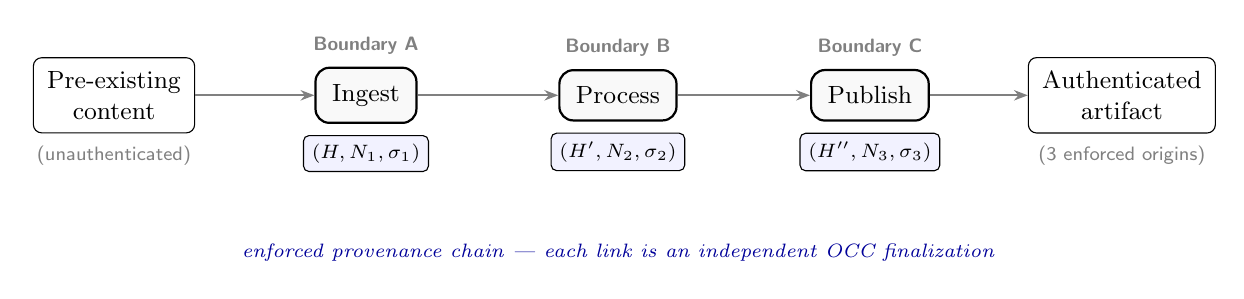
\begin{tikzpicture}[
  box/.style={draw, rounded corners=3pt, minimum height=0.8cm, align=center,
              font=\small, inner sep=5pt},
  bnd/.style={draw, thick, rounded corners=5pt, fill=gray!5, align=center,
              font=\small, inner sep=6pt},
  proof/.style={fill=blue!5, draw, rounded corners=2pt, font=\scriptsize\ttfamily,
                inner sep=3pt},
  arr/.style={-{Stealth[length=5pt]}, gray, thick},
  lbl/.style={font=\scriptsize\sffamily, text=gray},
]
\node[box] (pre) at (0,0) {Pre-existing\\content};
\node[lbl, below=1pt of pre] {(unauthenticated)};

\node[bnd] (ba) at (3.2,0) {Ingest};
\node[lbl, above=1pt of ba] {\textbf{\sffamily Boundary A}};
\node[proof, below=4pt of ba] {$(H, N_1, \sigma_1)$};

\node[bnd] (bb) at (6.4,0) {Process};
\node[lbl, above=1pt of bb] {\textbf{\sffamily Boundary B}};
\node[proof, below=4pt of bb] {$(H', N_2, \sigma_2)$};

\node[bnd] (bc) at (9.6,0) {Publish};
\node[lbl, above=1pt of bc] {\textbf{\sffamily Boundary C}};
\node[proof, below=4pt of bc] {$(H'', N_3, \sigma_3)$};

\node[box] (final) at (12.8,0) {Authenticated\\artifact};
\node[lbl, below=1pt of final] {(3 enforced origins)};

\draw[arr] (pre) -- (ba);
\draw[arr] (ba) -- (bb);
\draw[arr] (bb) -- (bc);
\draw[arr] (bc) -- (final);

\node[font=\scriptsize\itshape, blue!60!black] at (6.4,-2)
  {enforced provenance chain --- each link is an independent OCC finalization};
\end{tikzpicture}
\caption{Enforced provenance chains. Pre-existing content traverses multiple OCC boundaries, each producing independent verification material. Each admission is a separate enforced finalization event. The resulting chain is structurally guaranteed---not voluntarily annotated---because each link requires traversal of a protected commit interface.}
\label{fig:provenance-chains}
\end{figure}


% ============================================================================
% 14. IMPLEMENTATION CONSIDERATIONS
% ============================================================================
\section{Implementation Considerations}
\label{sec:implementation}

\paragraph{Latency.}
Creation-time enforcement must be fast enough to run on capture and export paths without degrading user experience or pipeline throughput. Efficient proof generation and verification are engineering constraints, not architectural limitations. Modern signing operations (Ed25519, ECDSA P-256) complete in microseconds on current hardware.

\paragraph{Offline operation.}
Environments requiring offline creation can generate proofs locally and defer admission into trusted domains until connectivity is available. Trusted domains then enforce verification at ingestion. This provides bounded issuance guarantees rather than continuous supervision---analogous to how physical secure instruments (e.g., pre-signed checks) operate with deferred clearing. In extreme cases---interplanetary missions, remote sensor networks, or disconnected autonomous systems---offline operation may span hours to days, with proofs verified only upon eventual receipt at a ground station or gateway operating under the same trust anchors.

\paragraph{Failure handling.}
Systems must define failure behavior. For high-assurance domains, fail-closed behavior is required: if proof generation fails, finalization is blocked. For consumer deployments, staged enforcement may begin with fail-open at selected boundaries and evolve toward fail-closed as operational confidence increases.

\paragraph{Verification material formats and transport.}
Verification material may be embedded within the artifact, carried in a sidecar file, included in a bundle manifest, transmitted as an authenticated envelope, or held at a reference point for query-based verification (see \cref{sec:verification-independence}). The key requirement is that verification material is bound to the artifact in a way that can be validated independently and cannot be retroactively attached without detection. The choice of transport mechanism is a deployment decision; the enforcement invariant is the same regardless of how verification material reaches the verifier.

\paragraph{Key rotation and revocation.}
Operational deployments require key rotation policies and revocation mechanisms. When a boundary is compromised, trust anchors can be revoked or rotated, new boundary identities introduced, and epoch constraints enforced on acceptable verification material. No artifact registry is required for rotation or recovery.

\paragraph{Interoperability with provenance systems.}
OCC coexists with provenance and credentialing systems that focus on post-creation traceability. Provenance chains can be attached to artifacts finalized under OCC, providing richer downstream traceability. The admission decision remains anchored in enforced finalization, while provenance provides the interoperability layer for distribution and audit.


% ============================================================================
% 15. DEPLOYMENT
% ============================================================================
\section{Deployment and Adoption}
\label{sec:deployment}

Origin Controlled Computing is best understood as an enforcement primitive that can be introduced incrementally. Most environments cannot transition from fully permissive creation to strict admissibility in a single step.

\paragraph{Phased rollout.}
A practical deployment begins with visibility: attaching verification material when available and surfacing authenticated versus unauthenticated status. The next phase requires authenticated finalization for selected high-assurance workflows while allowing unauthenticated outputs in a separate untrusted lane. Over time, enforcement expands to additional repositories, export paths, and regulated domains. Each phase requires engineering integration with existing commit paths, and the phased model is designed to contain this cost by limiting initial enforcement to high-value boundaries.

\paragraph{Policy-driven boundaries.}
The decisive question in most deployments is not whether an artifact can be produced, but whether it can be admitted into a domain that confers legitimacy, downstream impact, or compliance standing. OCC can be applied selectively at these boundaries: ingestion into training corpora, publication to official channels, archival in compliance systems, or persistence into audit-grade logs.

\paragraph{Institutional adoption incentives.}
Adoption is accelerated when benefits are concrete: reduced downstream moderation burden, improved auditability, clearer liability boundaries, and the ability to define and enforce admissible content policies. In high-volume environments, the ability to reject unauthenticated artifacts at ingestion is more valuable than attempting to detect or classify them after the fact. Organizations already subject to compliance mandates---regulated data processors, evidentiary systems, and entities operating under frameworks such as the EU AI Act---are natural early adopters, as they face the strongest immediate demand for structural authenticity guarantees.

\paragraph{End state.}
The end state is not universal prevention of unauthenticated creation, but reliable exclusion of unauthenticated durable state from the systems and pipelines where legitimacy, compliance, and downstream impact are determined.


% ============================================================================
% 16. APPLICATIONS
% ============================================================================
\section{Applications}
\label{sec:applications}

Origin Controlled Computing applies wherever systems must distinguish admissible durable outputs from arbitrary durable outputs produced outside trusted pipelines. The common architectural pattern is a protected commit path that gates admission into authenticated durable state. The pattern arises across domains:

\begin{enumerate}
  \item \textbf{AI training and inference pipelines}, where only authenticated outputs may be admitted into datasets or downstream automation.
  \item \textbf{Media capture and evidentiary systems}, where admissibility depends on verified creation conditions.
  \item \textbf{Compliance logging and telemetry}, where audit records must resist post-hoc fabrication.
  \item \textbf{Scientific instruments and simulations}, where experimental results must be traceable to controlled execution environments.
  \item \textbf{Regulated data processing} in finance, healthcare, safety monitoring, and government systems.
  \item \textbf{Digital identity and credential issuance}, where credentials must be structurally unforgeable.
  \item \textbf{Supply chain verification}, where provenance must be enforced at each handoff rather than reconstructed afterward.
  \item \textbf{Authorization transfer and ledger-independent scarcity}, where transfer of digital value or authority is enforced by a single atomic transition that both irreversibly de-authorizes the sender capability and generates the receiver capability within a protected execution boundary. This is a direct application of the birth--death semantics described in \cref{sec:birth-death}: the prior authority undergoes verifiable death, and the successor undergoes verifiable birth, within a single atomic event. This preserves scarcity invariants structurally and implies double-spend resistance without global ledgers, distributed consensus, or registry-based settlement infrastructure. The settlement and monetary implications are substantial and are explored separately.
  \item \textbf{Interplanetary and delay-tolerant systems}, where authentication must be non-interactive, verification must occur offline, and proofs must travel with data across store-and-forward networks with minutes-to-hours latency. OCC's non-interactive finalization, compact portable proofs, and hardware-rooted trust align with the operational constraints of DTN/Bundle Protocol environments, where real-time protocols, centralized registries, and consensus mechanisms are infeasible.
\end{enumerate}

Across these domains, trust derives from enforced admission into authenticated state at commit time, not from retrospective provenance reconstruction. When admissibility matters, origin enforcement necessarily moves into the creation and finalization paths of the system.


% ============================================================================
% 17. BIRTH-DEATH SEMANTICS
% ============================================================================
\section{Birth--Death Semantics}
\label{sec:birth-death}

Origin Controlled Computing (OCC) enforces what we term \emph{birth--death semantics} for digital state. Under this model, every authoritative state transition has exactly one verifiable moment of creation (birth), and every transfer or succession requires cryptographic evidence that the prior authority has been irreversibly consumed (death).

Traditional provenance systems operate in a \emph{detect-after} model: artifacts are produced freely, and conflicts such as replay, duplication, or double-spend are identified retrospectively through logs, ledgers, or consensus. OCC instead constrains the execution path such that invalid successor states are structurally unreachable within the enforcing boundary.

% ---------- Figure 7: Birth-Death Semantics ----------
\begin{figure}[htbp]
\centering
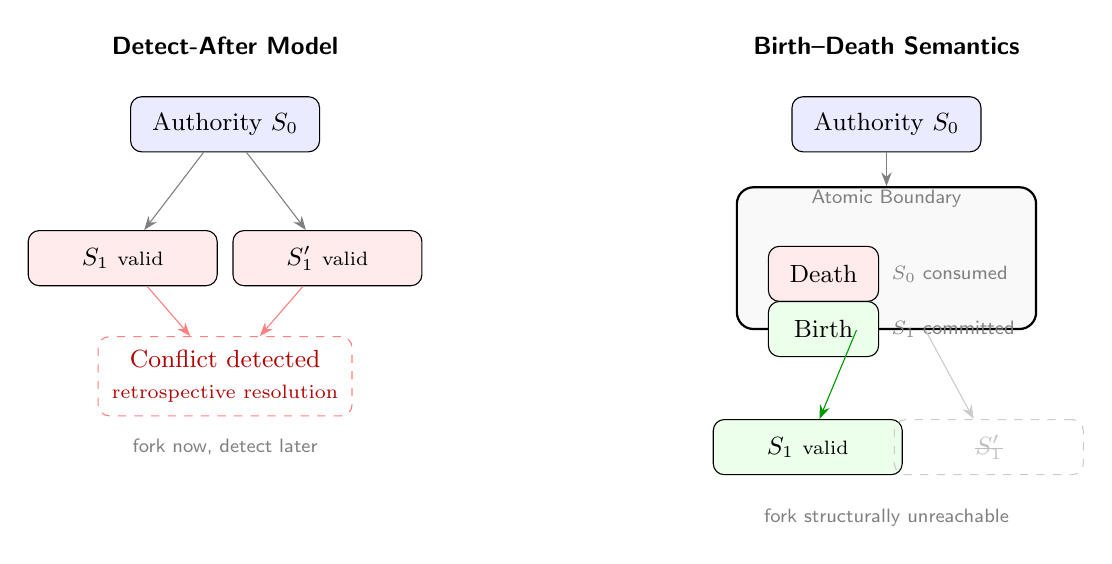
\begin{tikzpicture}[
  box/.style={draw, rounded corners=4pt, minimum width=2.4cm, minimum height=0.7cm,
              align=center, font=\small, inner sep=5pt},
  bndbox/.style={draw, thick, rounded corners=6pt, fill=gray!5, inner sep=8pt},
  arr/.style={-{Stealth[length=5pt]}, gray},
  lbl/.style={font=\scriptsize\sffamily, text=gray},
]
% --- Left: Detect-After ---
\node[font=\small\bfseries\sffamily] at (-4.2,4.5) {Detect-After Model};
\node[box, fill=blue!8] (da0) at (-4.2,3.5) {Authority $S_0$};
\node[box, fill=red!8] (da1) at (-5.5,1.8) {$S_1$ {\scriptsize valid}};
\node[box, fill=red!8] (da1p) at (-2.9,1.8) {$S_1'$ {\scriptsize valid}};
\draw[arr] (da0) -- (da1);
\draw[arr] (da0) -- (da1p);
\node[box, draw=red!50, dashed, text=red!70!black] (conflict) at (-4.2,0.3)
  {Conflict detected\\{\scriptsize retrospective resolution}};
\draw[arr, red!50] (da1) -- (conflict);
\draw[arr, red!50] (da1p) -- (conflict);
\node[lbl] at (-4.2,-0.6) {fork now, detect later};

% --- Right: Birth-Death ---
\node[font=\small\bfseries\sffamily] at (4.2,4.5) {Birth--Death Semantics};
\node[box, fill=blue!8] (bd0) at (4.2,3.5) {Authority $S_0$};

\node[bndbox, minimum width=3.8cm, minimum height=1.8cm] (bdbox) at (4.2,1.8) {};
\node[lbl] at (4.2,2.55) {Atomic Boundary};
\node[box, fill=red!8, minimum width=1.4cm] (death) at (3.4,1.6) {Death};
\node[lbl, right=1pt of death] {$S_0$ consumed};
\node[box, fill=green!8, minimum width=1.4cm] (birth) at (3.4,0.9) {Birth};
\node[lbl, right=1pt of birth] {$S_1$ committed};

\draw[arr] (bd0) -- (bdbox);

\node[box, fill=green!8] (bd1) at (3.2,-0.6) {$S_1$ {\scriptsize valid}};
\node[box, draw=gray!40, dashed, text=gray!50, font=\small] (bd1p) at (5.5,-0.6)
  {\sout{$S_1'$}};

\draw[arr, green!60!black] (bdbox) -- (bd1);
\draw[arr, gray!40] (bdbox) -- (bd1p);

\node[lbl] at (4.2,-1.5) {fork structurally unreachable};
\end{tikzpicture}
\caption{Detect-after vs.\ birth--death enforcement. Traditional systems (left) permit both successor states to be produced and detect conflicts retrospectively. Under birth--death semantics (right), the prior authority is irreversibly consumed within the atomic boundary, and exactly one successor is committed. The alternative fork is not merely unlikely---it is structurally unreachable within the enforcing boundary.}
\label{fig:birth-death}
\end{figure}


% --- 17.1 ---
\subsection{Construction}
\label{sec:bd-construction}

Within a verifier-accepted measured boundary (e.g., a Trusted Execution Environment or equivalent protected constructor), a valid OCC commit requires the atomic execution of the following steps:
\begin{itemize}
  \item Policy authorization of the requested operation
  \item Generation and atomic consumption of a fresh, non-replayable commitment value (either an unpredictable nonce or a strictly monotonic counter)
  \item Collision-resistant binding of the artifact digest to the consumed value
  \item Durable commit of the resulting signed proof
\end{itemize}

No intermediate state is externally observable, and partial completion yields no valid proof. The consumed value establishes a forward-only lineage: any valid successor must reference a strictly later state within the boundary's monotonic domain.


% --- 17.2 ---
\subsection{Single-Successor Property}
\label{sec:bd-single-successor}

Given correct enforcement of measurement and monotonicity within the boundary, OCC guarantees:

\begin{property}[Single-Successor]
\label{prop:single-successor}
At most one valid successor can be produced from any given parent authority within the verifier-accepted measurement and monotonicity domain of the enforcing boundary.
\end{property}

If two purported successors are observed downstream, at least one of the following must hold:
\begin{itemize}
  \item The enforcing boundary was compromised or misconfigured
  \item Monotonic state or anti-rollback guarantees were violated
  \item The verifier accepted an out-of-policy measurement
  \item The usage context exceeded the declared trust model
\end{itemize}

This reframes failure analysis from probabilistic conflict resolution to deterministic boundary integrity verification.


% --- 17.3 ---
\subsection{Relationship to Double-Spend}
\label{sec:bd-double-spend}

Birth--death semantics targets the core primitive underlying double-spend failures: the ability to produce multiple valid successor states from a single authority. By making such forks structurally unreachable at commit time within the stated trust envelope, OCC reduces reliance on global ordering for single-holder and provenance-sensitive workflows.

OCC does not claim global uniqueness across mutually distrustful, permissionless environments without additional coordination. Instead, it provides strong local authority guarantees that higher-level systems may compose with federation or consensus where global agreement is required.


% --- 17.4 ---
\subsection{Trust Envelope}
\label{sec:bd-trust-envelope}

The guarantees above hold only within the verifier-accepted measurement and monotonicity domain of the enforcing boundary. In particular:
\begin{itemize}
  \item A protected execution boundary is required for enforcement
  \item Monotonic state must be resistant to rollback within that boundary
  \item Verifiers must enforce measurement policy and counter monotonicity
  \item OCC does not prevent byte-level copying of artifacts outside the authority model
\end{itemize}

Within this envelope, birth--death semantics converts post-facto detection problems into construction-time exclusion properties.


% ============================================================================
% 18. SINGLE-TRANSFER VALUE WITHOUT CONSENSUS
% ============================================================================
\section{Single-Transfer Value Without Consensus}
\label{sec:value-transfer}

Origin Controlled Computing (OCC) enables single-transfer digital value by binding authority to a consumptive, cryptographically enforced state transition rather than to a ledger entry. This is a concrete instantiation of the birth--death semantics described in \cref{sec:birth-death}: each transfer atomically consumes (kills) the prior holder's authority and produces (births) a new verifiable successor. Each artifact carries a proof that can only be produced through a protected commit path, where authorization, binding, and durable commit occur atomically inside a trusted execution boundary. When value is transferred, the prior holder's permission is provably consumed and the new state is independently verifiable offline using public keys and hash lineage. The bytes themselves may be copied, but the authoritative right cannot be duplicated, because the single-successor property guarantees that only one unspent lineage can exist at a time within the enforcing boundary. In this model, uniqueness and transfer integrity come from enforced execution semantics instead of global consensus, allowing blockchain-free, verifiable digital handoff.


% ============================================================================
% 19. CONCLUSION
% ============================================================================
\section{Conclusion}
\label{sec:conclusion}

The Trusted Origin Token Architecture demonstrates that origin control can be enforced by consuming authorization units at finalization. Origin Controlled Computing generalizes this result by showing that equivalent enforcement is achieved using boundary-fresh cryptographic computation and protected commit paths, without requiring tracked tokens.

Atomic Causality links authorization, cryptographic binding, and durable commit into a single indivisible event. Authenticated durable state is defined by structural reachability---by the state transitions that produced it---not by historical claims, metadata, or post-hoc annotation.

The formal model presented here shows that OCC defines a new enforcement primitive: a \emph{genesis access control mechanism} that constrains which authenticated objects are permitted to exist, rather than mediating operations on objects that already exist. This is strictly stronger than classical reference monitors and formally distinct from attested execution, information flow control, and capability-based security.

By securing creation rather than history, Origin Controlled Computing establishes an architectural primitive for trustworthy digital systems. It does not replace provenance, verification, or access control. It provides the structural foundation that makes those mechanisms enforceable at the boundaries where legitimacy is conferred.


% ============================================================================
% REFERENCES
% ============================================================================
\begin{thebibliography}{17}

\bibitem{anderson1972}
J.~P. Anderson,
``Computer security technology planning study,''
Tech.\ Rep.\ ESD-TR-73-51, Electronic Systems Division, AFSC, 1972.

\bibitem{arms2000}
W.~Y. Arms,
\emph{Digital Libraries},
MIT Press, 2000.

\bibitem{c2pa2024}
Coalition for Content Provenance and Authenticity (C2PA),
``C2PA Technical Specification v2.1,'' 2024.

\bibitem{costan2016}
V.~Costan and S.~Devadas,
``Intel SGX explained,''
IACR Cryptology ePrint Archive, Report 2016/086, 2016.

\bibitem{dennis1966}
J.~B. Dennis and E.~C. Van Horn,
``Programming semantics for multiprogrammed computations,''
\emph{Communications of the ACM}, vol.~9, no.~3, pp.~143--155, 1966.

\bibitem{dice2020}
Trusted Computing Group,
``DICE Layered Architecture,'' 2020.

\bibitem{goguen1982}
J.~A. Goguen and J.~Meseguer,
``Security policies and security models,''
in \emph{Proc.\ IEEE Symposium on Security and Privacy}, pp.~11--20, 1982.

\bibitem{green2007}
T.~J. Green, G.~Karvounarakis, and V.~Tannen,
``Provenance semirings,''
in \emph{Proc.\ ACM SIGMOD-SIGACT-SIGART Symposium on Principles of Database Systems (PODS)}, pp.~31--40, 2007.

\bibitem{ietf2023}
IETF,
``Remote ATtestation procedureS (RATS) Architecture,''
RFC 9334, 2023.

\bibitem{jones1983}
C.~B. Jones,
``Tentative steps toward a development method for interfering programs,''
\emph{ACM Transactions on Programming Languages and Systems}, vol.~5, no.~4, pp.~596--619, 1983.

\bibitem{lampson1971}
B.~W. Lampson,
``Protection,''
in \emph{Proc.\ 5th Princeton Symposium on Information Sciences and Systems}, pp.~437--443, 1971.

\bibitem{miller2006}
M.~S. Miller,
``Robust composition: Towards a unified approach to access control and concurrency control,''
Ph.D.\ dissertation, Johns Hopkins University, 2006.

\bibitem{myers1997}
A.~C. Myers and B.~Liskov,
``A decentralized model for information flow control,''
in \emph{Proc.\ 16th ACM Symposium on Operating Systems Principles (SOSP)}, pp.~129--142, 1997.

\bibitem{necula1997}
G.~C. Necula,
``Proof-carrying code,''
in \emph{Proc.\ 24th ACM SIGPLAN-SIGACT Symposium on Principles of Programming Languages (POPL)}, pp.~106--119, 1997.

\bibitem{burleigh2007}
S.~Burleigh, K.~Fall, and V.~Cerf,
``Delay-Tolerant Networking Architecture,''
RFC 4838, 2007.

\bibitem{scott2022}
K.~Scott, S.~Burleigh, et~al.,
``Bundle Protocol Version 7,''
RFC 9171, 2022.

\bibitem{birrane2022}
E.~Birrane~III and K.~McKeever,
``Bundle Protocol Security (BPSec),''
RFC 9172, 2022.

\end{thebibliography}

\end{document}
